\documentclass{book}
\usepackage[a4paper,top=2.5cm,bottom=2.5cm,left=2.5cm,right=2.5cm]{geometry}
\usepackage{makeidx}
\usepackage{natbib}
\usepackage{graphicx}
\usepackage{multicol}
\usepackage{float}
\usepackage{listings}
\usepackage{color}
\usepackage{ifthen}
\usepackage[table]{xcolor}
\usepackage{textcomp}
\usepackage{alltt}
\usepackage{ifpdf}
\ifpdf
\usepackage[pdftex,
            pagebackref=true,
            colorlinks=true,
            linkcolor=blue,
            unicode
           ]{hyperref}
\else
\usepackage[ps2pdf,
            pagebackref=true,
            colorlinks=true,
            linkcolor=blue,
            unicode
           ]{hyperref}
\usepackage{pspicture}
\fi
\usepackage[utf8]{inputenc}
\usepackage{mathptmx}
\usepackage[scaled=.90]{helvet}
\usepackage{courier}
\usepackage{sectsty}
\usepackage[titles]{tocloft}
\usepackage{doxygen}
\lstset{language=C++,inputencoding=utf8,basicstyle=\footnotesize,breaklines=true,breakatwhitespace=true,tabsize=4,numbers=left }
\makeindex
\setcounter{tocdepth}{3}
\renewcommand{\footrulewidth}{0.4pt}
\renewcommand{\familydefault}{\sfdefault}
\hfuzz=15pt
\setlength{\emergencystretch}{15pt}
\hbadness=750
\tolerance=750
\begin{document}
\hypersetup{pageanchor=false,citecolor=blue}
\begin{titlepage}
\vspace*{7cm}
\begin{center}
{\Large e\-Z Advanced Autoload \\[1ex]\large 1.\-0.\-0-\/\-R\-C }\\
\vspace*{1cm}
{\large Generated by Doxygen 1.8.0}\\
\vspace*{0.5cm}
{\small Fri Mar 9 2012 14:57:39}\\
\end{center}
\end{titlepage}
\clearemptydoublepage
\pagenumbering{roman}
\tableofcontents
\clearemptydoublepage
\pagenumbering{arabic}
\hypersetup{pageanchor=true,citecolor=blue}
\chapter{Todo List}
\label{todo}
\hypertarget{todo}{}

\begin{DoxyRefList}
\item[\label{todo__todo000002}%
\hypertarget{todo__todo000002}{}%
\-Member \hyperlink{classextension_1_1ezadvancedautoload_1_1pv_1_1classes_1_1e_z_autoload_generator_a2556d8c52deb73d88fb2eff9342a7237}{extension} (\$path)]put this in a real helper  
\item[\label{todo__todo000001}%
\hypertarget{todo__todo000001}{}%
\-Member \hyperlink{classextension_1_1ezadvancedautoload_1_1pv_1_1classes_1_1e_z_autoload_generator_afd315c7aa866c6a1bfcf75ae27ce8c3b}{extension} ()]put this in a real helper 
\end{DoxyRefList}
\chapter{Namespace Index}
\section{\-Packages}
\-Here are the packages with brief descriptions (if available)\-:\begin{DoxyCompactList}
\item\contentsline{section}{\hyperlink{namespaceextension}{extension} \\*\-Enumeration class for autoload generator }{\pageref{namespaceextension}}{}
\item\contentsline{section}{\hyperlink{namespaceextension_1_1ezadvancedautoload}{extension\-::ezadvancedautoload} }{\pageref{namespaceextension_1_1ezadvancedautoload}}{}
\item\contentsline{section}{\hyperlink{namespaceextension_1_1ezadvancedautoload_1_1classes}{extension\-::ezadvancedautoload\-::classes} }{\pageref{namespaceextension_1_1ezadvancedautoload_1_1classes}}{}
\item\contentsline{section}{\hyperlink{namespaceextension_1_1ezadvancedautoload_1_1classes_1_1enums}{extension$\backslash$ezadvancedautoload$\backslash$classes$\backslash$enums} }{\pageref{namespaceextension_1_1ezadvancedautoload_1_1classes_1_1enums}}{}
\item\contentsline{section}{\hyperlink{namespaceextension_1_1ezadvancedautoload_1_1classes_1_1exceptions}{extension$\backslash$ezadvancedautoload$\backslash$classes$\backslash$exceptions} }{\pageref{namespaceextension_1_1ezadvancedautoload_1_1classes_1_1exceptions}}{}
\item\contentsline{section}{\hyperlink{namespaceextension_1_1ezadvancedautoload_1_1classes_1_1helpers}{extension$\backslash$ezadvancedautoload$\backslash$classes$\backslash$helpers} }{\pageref{namespaceextension_1_1ezadvancedautoload_1_1classes_1_1helpers}}{}
\item\contentsline{section}{\hyperlink{namespaceextension_1_1ezadvancedautoload_1_1pv}{extension\-::ezadvancedautoload\-::pv} }{\pageref{namespaceextension_1_1ezadvancedautoload_1_1pv}}{}
\item\contentsline{section}{\hyperlink{namespaceextension_1_1ezadvancedautoload_1_1pv_1_1classes}{extension$\backslash$ezadvancedautoload$\backslash$pv$\backslash$classes} }{\pageref{namespaceextension_1_1ezadvancedautoload_1_1pv_1_1classes}}{}
\end{DoxyCompactList}

\chapter{Data Structure Index}
\section{Class Hierarchy}
This inheritance list is sorted roughly, but not completely, alphabetically\-:\begin{DoxyCompactList}
\item \contentsline{section}{extension$\backslash$ezadvancedautoload$\backslash$classes$\backslash$enums$\backslash$autoload\-Generator\-Enum}{\pageref{classextension_1_1ezadvancedautoload_1_1classes_1_1enums_1_1autoload_generator_enum}}{}
\item \contentsline{section}{extension$\backslash$ezadvancedautoload$\backslash$pv$\backslash$classes$\backslash$e\-Z\-Autoload\-Generator}{\pageref{classextension_1_1ezadvancedautoload_1_1pv_1_1classes_1_1e_z_autoload_generator}}{}
\item \contentsline{section}{extension$\backslash$ezadvancedautoload$\backslash$classes$\backslash$helpers$\backslash$Helper}{\pageref{classextension_1_1ezadvancedautoload_1_1classes_1_1helpers_1_1_helper}}{}
\begin{DoxyCompactList}
\item \contentsline{section}{extension$\backslash$ezadvancedautoload$\backslash$classes$\backslash$helpers$\backslash$template\-Autoload\-Generator\-Helper}{\pageref{classextension_1_1ezadvancedautoload_1_1classes_1_1helpers_1_1template_autoload_generator_helper}}{}
\end{DoxyCompactList}
\item \contentsline{section}{extension$\backslash$ezadvancedautoload$\backslash$classes$\backslash$exceptions$\backslash$unexpected\-Mode\-Exception}{\pageref{classextension_1_1ezadvancedautoload_1_1classes_1_1exceptions_1_1unexpected_mode_exception}}{}
\end{DoxyCompactList}

\chapter{Data Structure Index}
\section{Data Structures}
Here are the data structures with brief descriptions\-:\begin{DoxyCompactList}
\item\contentsline{section}{\hyperlink{classextension_1_1ezadvancedautoload_1_1classes_1_1enums_1_1autoload_generator_enum}{extension$\backslash$ezadvancedautoload$\backslash$classes$\backslash$enums$\backslash$autoload\-Generator\-Enum} }{\pageref{classextension_1_1ezadvancedautoload_1_1classes_1_1enums_1_1autoload_generator_enum}}{}
\item\contentsline{section}{\hyperlink{classextension_1_1ezadvancedautoload_1_1pv_1_1classes_1_1e_z_autoload_generator}{extension$\backslash$ezadvancedautoload$\backslash$pv$\backslash$classes$\backslash$e\-Z\-Autoload\-Generator} }{\pageref{classextension_1_1ezadvancedautoload_1_1pv_1_1classes_1_1e_z_autoload_generator}}{}
\item\contentsline{section}{\hyperlink{classextension_1_1ezadvancedautoload_1_1classes_1_1helpers_1_1_helper}{extension$\backslash$ezadvancedautoload$\backslash$classes$\backslash$helpers$\backslash$\-Helper} }{\pageref{classextension_1_1ezadvancedautoload_1_1classes_1_1helpers_1_1_helper}}{}
\item\contentsline{section}{\hyperlink{classextension_1_1ezadvancedautoload_1_1classes_1_1helpers_1_1template_autoload_generator_helper}{extension$\backslash$ezadvancedautoload$\backslash$classes$\backslash$helpers$\backslash$template\-Autoload\-Generator\-Helper} }{\pageref{classextension_1_1ezadvancedautoload_1_1classes_1_1helpers_1_1template_autoload_generator_helper}}{}
\item\contentsline{section}{\hyperlink{classextension_1_1ezadvancedautoload_1_1classes_1_1exceptions_1_1unexpected_mode_exception}{extension$\backslash$ezadvancedautoload$\backslash$classes$\backslash$exceptions$\backslash$unexpected\-Mode\-Exception} }{\pageref{classextension_1_1ezadvancedautoload_1_1classes_1_1exceptions_1_1unexpected_mode_exception}}{}
\end{DoxyCompactList}

\chapter{File Index}
\section{File List}
Here is a list of all files with brief descriptions\-:\begin{DoxyCompactList}
\item\contentsline{section}{C\-:/\-Users/aloyant/ezadvancedautoload/bin/php/\hyperlink{ezpgenerateautoloads_8php}{ezpgenerateautoloads.\-php} }{\pageref{ezpgenerateautoloads_8php}}{}
\item\contentsline{section}{C\-:/\-Users/aloyant/ezadvancedautoload/classes/enums/\hyperlink{autoloadgeneratorenum_8php}{autoloadgeneratorenum.\-php} }{\pageref{autoloadgeneratorenum_8php}}{}
\item\contentsline{section}{C\-:/\-Users/aloyant/ezadvancedautoload/classes/exceptions/\hyperlink{unexpectedmodeexception_8php}{unexpectedmodeexception.\-php} }{\pageref{unexpectedmodeexception_8php}}{}
\item\contentsline{section}{C\-:/\-Users/aloyant/ezadvancedautoload/classes/helpers/\hyperlink{helper_8php}{helper.\-php} }{\pageref{helper_8php}}{}
\item\contentsline{section}{C\-:/\-Users/aloyant/ezadvancedautoload/classes/helpers/\hyperlink{templateautoloadgeneratorhelper_8php}{templateautoloadgeneratorhelper.\-php} }{\pageref{templateautoloadgeneratorhelper_8php}}{}
\item\contentsline{section}{C\-:/\-Users/aloyant/ezadvancedautoload/doc/examples/\hyperlink{call__regenerate__helper_8php}{call\-\_\-regenerate\-\_\-helper.\-php} }{\pageref{call__regenerate__helper_8php}}{}
\item\contentsline{section}{C\-:/\-Users/aloyant/ezadvancedautoload/modules/ezadvancedautoload/\hyperlink{extensions_8php}{extensions.\-php} }{\pageref{extensions_8php}}{}
\item\contentsline{section}{C\-:/\-Users/aloyant/ezadvancedautoload/modules/ezadvancedautoload/\hyperlink{module_8php}{module.\-php} }{\pageref{module_8php}}{}
\item\contentsline{section}{C\-:/\-Users/aloyant/ezadvancedautoload/private/classes/\hyperlink{ezautoloadgenerator_8php}{ezautoloadgenerator.\-php} }{\pageref{ezautoloadgenerator_8php}}{}
\item\contentsline{section}{C\-:/\-Users/aloyant/ezadvancedautoload/settings/\hyperlink{autoload_8ini_8append_8php}{autoload.\-ini.\-append.\-php} }{\pageref{autoload_8ini_8append_8php}}{}
\item\contentsline{section}{C\-:/\-Users/aloyant/ezadvancedautoload/settings/\hyperlink{design_8ini_8append_8php}{design.\-ini.\-append.\-php} }{\pageref{design_8ini_8append_8php}}{}
\item\contentsline{section}{C\-:/\-Users/aloyant/ezadvancedautoload/settings/\hyperlink{module_8ini_8append_8php}{module.\-ini.\-append.\-php} }{\pageref{module_8ini_8append_8php}}{}
\item\contentsline{section}{C\-:/\-Users/aloyant/ezadvancedautoload/settings/\hyperlink{site_8ini_8append_8php}{site.\-ini.\-append.\-php} }{\pageref{site_8ini_8append_8php}}{}
\end{DoxyCompactList}

\chapter{Namespace Documentation}
\hypertarget{namespaceextension}{\section{extension Namespace Reference}
\label{namespaceextension}\index{extension@{extension}}
}


Enumeration class for autoload generator.  


\subsection*{Namespaces}
\begin{DoxyCompactItemize}
\item 
namespace \hyperlink{namespaceextension_1_1ezadvancedautoload}{ezadvancedautoload}
\end{DoxyCompactItemize}


\subsection{Detailed Description}
Enumeration class for autoload generator. File containing the e\-Z\-Autoload\-Generator class.

Helper witch provide help to correctly build autoload file.

Meta class for all helpers.

Unexpected\-Mode\-Exception class.

Classe witch define all enumeration use for build autoload This class will need to extends \href{http://php.net/manual/fr/book.spl-types.php}{\tt Spl\-Enum} soon It's a final class because there is no need to extends it; It should manage all available parameter for autoload generation with e\-Z\-Publish

\begin{DoxyAuthor}{Author}
Adrien Loyant \href{mailto:adrien.loyant@te-laval.fr}{\tt adrien.\-loyant@te-\/laval.\-fr}
\end{DoxyAuthor}
\begin{DoxyDate}{Date}
2012-\/03-\/01 
\end{DoxyDate}
\begin{DoxyVersion}{Version}
1.\-0.\-0 
\end{DoxyVersion}
\begin{DoxySince}{Since}
1.\-0.\-0 
\end{DoxySince}
\begin{DoxyCopyright}{Copyright}
G\-N\-U Public License v.\-2
\end{DoxyCopyright}


Unexpected\-Mode\-Exception class for throwing exception when the mode for autoload generation is not correct

\begin{DoxyAuthor}{Author}
Adrien Loyant \href{mailto:adrien.loyant@te-laval.fr}{\tt adrien.\-loyant@te-\/laval.\-fr}
\end{DoxyAuthor}
\begin{DoxyDate}{Date}
2012-\/03-\/01 
\end{DoxyDate}
\begin{DoxyVersion}{Version}
1.\-0.\-0 
\end{DoxyVersion}
\begin{DoxySince}{Since}
1.\-0.\-0 
\end{DoxySince}
\begin{DoxyCopyright}{Copyright}
G\-N\-U Public License v.\-2
\end{DoxyCopyright}


All helper classes should extends this class because this is their Meta\-Class

\begin{DoxyAuthor}{Author}
Adrien Loyant \href{mailto:adrien.loyant@te-laval.fr}{\tt adrien.\-loyant@te-\/laval.\-fr}
\end{DoxyAuthor}
\begin{DoxyDate}{Date}
2012-\/03-\/01 
\end{DoxyDate}
\begin{DoxyVersion}{Version}
1.\-0.\-0 
\end{DoxyVersion}
\begin{DoxySince}{Since}
1.\-0.\-0 
\end{DoxySince}
\begin{DoxyCopyright}{Copyright}
G\-N\-U Public License v.\-2
\end{DoxyCopyright}


Helper witch provide help to correctly build autoload file

\begin{DoxyAuthor}{Author}
Adrien Loyant \href{mailto:adrien.loyant@te-laval.fr}{\tt adrien.\-loyant@te-\/laval.\-fr}
\end{DoxyAuthor}
\begin{DoxyDate}{Date}
2012-\/03-\/01 
\end{DoxyDate}
\begin{DoxyVersion}{Version}
1.\-0.\-0 
\end{DoxyVersion}
\begin{DoxySince}{Since}
1.\-0.\-0 
\end{DoxySince}
\begin{DoxyCopyright}{Copyright}
G\-N\-U Public License v.\-2
\end{DoxyCopyright}


This class permits to generate autoload array without considering unactivated extensions

\begin{DoxyAuthor}{Author}
Adrien Loyant \href{mailto:adrien.loyant@te-laval.fr}{\tt adrien.\-loyant@te-\/laval.\-fr}
\end{DoxyAuthor}
\begin{DoxyDate}{Date}
2012-\/03-\/01 
\end{DoxyDate}
\begin{DoxyVersion}{Version}
1.\-0.\-0 
\end{DoxyVersion}
\begin{DoxySince}{Since}
1.\-0.\-0 
\end{DoxySince}
\begin{DoxyCopyright}{Copyright}
G\-N\-U Public License v.\-2
\end{DoxyCopyright}
\begin{DoxySeeAlso}{See also}

\end{DoxySeeAlso}

\hypertarget{namespaceextension_1_1ezadvancedautoload}{\section{extension$\backslash$ezadvancedautoload Namespace Reference}
\label{namespaceextension_1_1ezadvancedautoload}\index{extension$\backslash$ezadvancedautoload@{extension$\backslash$ezadvancedautoload}}
}
\subsection*{Namespaces}
\begin{DoxyCompactItemize}
\item 
namespace \hyperlink{namespaceextension_1_1ezadvancedautoload_1_1classes}{classes}
\item 
namespace \hyperlink{namespaceextension_1_1ezadvancedautoload_1_1pv}{pv}
\end{DoxyCompactItemize}

\hypertarget{namespaceextension_1_1ezadvancedautoload_1_1classes}{\section{extension\-:\-:ezadvancedautoload\-:\-:classes \-Namespace \-Reference}
\label{namespaceextension_1_1ezadvancedautoload_1_1classes}\index{extension\-::ezadvancedautoload\-::classes@{extension\-::ezadvancedautoload\-::classes}}
}
\subsection*{\-Packages}
\begin{DoxyCompactItemize}
\item 
namespace \hyperlink{namespaceextension_1_1ezadvancedautoload_1_1classes_1_1enums}{enums}
\item 
namespace \hyperlink{namespaceextension_1_1ezadvancedautoload_1_1classes_1_1exceptions}{exceptions}
\item 
namespace \hyperlink{namespaceextension_1_1ezadvancedautoload_1_1classes_1_1helpers}{helpers}
\end{DoxyCompactItemize}

\hypertarget{namespaceextension_1_1ezadvancedautoload_1_1classes_1_1enums}{\section{extension$\backslash$ezadvancedautoload$\backslash$classes$\backslash$enums Namespace Reference}
\label{namespaceextension_1_1ezadvancedautoload_1_1classes_1_1enums}\index{extension$\backslash$ezadvancedautoload$\backslash$classes$\backslash$enums@{extension$\backslash$ezadvancedautoload$\backslash$classes$\backslash$enums}}
}
\subsection*{Data Structures}
\begin{DoxyCompactItemize}
\item 
class \hyperlink{classextension_1_1ezadvancedautoload_1_1classes_1_1enums_1_1autoload_generator_enum}{autoload\-Generator\-Enum}
\end{DoxyCompactItemize}

\hypertarget{namespaceextension_1_1ezadvancedautoload_1_1classes_1_1exceptions}{\section{extension$\backslash$ezadvancedautoload$\backslash$classes$\backslash$exceptions Namespace Reference}
\label{namespaceextension_1_1ezadvancedautoload_1_1classes_1_1exceptions}\index{extension$\backslash$ezadvancedautoload$\backslash$classes$\backslash$exceptions@{extension$\backslash$ezadvancedautoload$\backslash$classes$\backslash$exceptions}}
}
\subsection*{Data Structures}
\begin{DoxyCompactItemize}
\item 
class \hyperlink{classextension_1_1ezadvancedautoload_1_1classes_1_1exceptions_1_1unexpected_mode_exception}{unexpected\-Mode\-Exception}
\end{DoxyCompactItemize}

\hypertarget{namespaceextension_1_1ezadvancedautoload_1_1classes_1_1helpers}{\section{extension$\backslash$ezadvancedautoload$\backslash$classes$\backslash$helpers \-Namespace \-Reference}
\label{namespaceextension_1_1ezadvancedautoload_1_1classes_1_1helpers}\index{extension$\backslash$ezadvancedautoload$\backslash$classes$\backslash$helpers@{extension$\backslash$ezadvancedautoload$\backslash$classes$\backslash$helpers}}
}
\subsection*{\-Classes}
\begin{DoxyCompactItemize}
\item 
class \hyperlink{classextension_1_1ezadvancedautoload_1_1classes_1_1helpers_1_1_helper}{\-Helper}
\item 
class \hyperlink{classextension_1_1ezadvancedautoload_1_1classes_1_1helpers_1_1template_autoload_generator_helper}{template\-Autoload\-Generator\-Helper}
\end{DoxyCompactItemize}

\hypertarget{namespaceextension_1_1ezadvancedautoload_1_1pv}{\section{extension$\backslash$ezadvancedautoload$\backslash$pv Namespace Reference}
\label{namespaceextension_1_1ezadvancedautoload_1_1pv}\index{extension$\backslash$ezadvancedautoload$\backslash$pv@{extension$\backslash$ezadvancedautoload$\backslash$pv}}
}
\subsection*{Namespaces}
\begin{DoxyCompactItemize}
\item 
namespace \hyperlink{namespaceextension_1_1ezadvancedautoload_1_1pv_1_1classes}{classes}
\end{DoxyCompactItemize}

\hypertarget{namespaceextension_1_1ezadvancedautoload_1_1pv_1_1classes}{\section{extension$\backslash$ezadvancedautoload$\backslash$pv$\backslash$classes Namespace Reference}
\label{namespaceextension_1_1ezadvancedautoload_1_1pv_1_1classes}\index{extension$\backslash$ezadvancedautoload$\backslash$pv$\backslash$classes@{extension$\backslash$ezadvancedautoload$\backslash$pv$\backslash$classes}}
}
\subsection*{Data Structures}
\begin{DoxyCompactItemize}
\item 
class \hyperlink{classextension_1_1ezadvancedautoload_1_1pv_1_1classes_1_1e_z_autoload_generator}{e\-Z\-Autoload\-Generator}
\end{DoxyCompactItemize}

\chapter{Data Structure Documentation}
\hypertarget{classextension_1_1ezadvancedautoload_1_1classes_1_1enums_1_1autoload_generator_enum}{\section{extension$\backslash$ezadvancedautoload$\backslash$classes$\backslash$enums$\backslash$autoload\-Generator\-Enum Class Reference}
\label{classextension_1_1ezadvancedautoload_1_1classes_1_1enums_1_1autoload_generator_enum}\index{extension$\backslash$ezadvancedautoload$\backslash$classes$\backslash$enums$\backslash$autoload\-Generator\-Enum@{extension$\backslash$ezadvancedautoload$\backslash$classes$\backslash$enums$\backslash$autoload\-Generator\-Enum}}
}
\subsection*{Data Fields}
\begin{DoxyCompactItemize}
\item 
const \hyperlink{classextension_1_1ezadvancedautoload_1_1classes_1_1enums_1_1autoload_generator_enum_aa803b338dcea315c5ba70ecdc103f306}{\-\_\-\-\_\-default} = self\-::\-E\-X\-T\-E\-N\-S\-I\-O\-N
\item 
const \hyperlink{classextension_1_1ezadvancedautoload_1_1classes_1_1enums_1_1autoload_generator_enum_a100ec557541f513d12bb988c9afdb99c}{K\-E\-R\-N\-E\-L} = 1
\item 
const \hyperlink{classextension_1_1ezadvancedautoload_1_1classes_1_1enums_1_1autoload_generator_enum_ab1c7c17892da9cd208eb3eb9ea4a55a4}{K\-E\-R\-N\-E\-L\-\_\-\-O\-V\-E\-R\-R\-I\-D\-E} = 2
\item 
const \hyperlink{classextension_1_1ezadvancedautoload_1_1classes_1_1enums_1_1autoload_generator_enum_a46f25431900773dbb0f22b71add686ce}{E\-X\-T\-E\-N\-S\-I\-O\-N} = 3
\item 
const \hyperlink{classextension_1_1ezadvancedautoload_1_1classes_1_1enums_1_1autoload_generator_enum_a7c160c4cf91bf4721a2ea9af96f4624a}{T\-E\-S\-T} = 4
\end{DoxyCompactItemize}


\subsection{Detailed Description}


Definition at line 20 of file autoloadgeneratorenum.\-php.



\subsection{Field Documentation}
\hypertarget{classextension_1_1ezadvancedautoload_1_1classes_1_1enums_1_1autoload_generator_enum_aa803b338dcea315c5ba70ecdc103f306}{\index{extension\-::ezadvancedautoload\-::classes\-::enums\-::autoload\-Generator\-Enum@{extension\-::ezadvancedautoload\-::classes\-::enums\-::autoload\-Generator\-Enum}!\-\_\-\-\_\-default@{\-\_\-\-\_\-default}}
\index{\-\_\-\-\_\-default@{\-\_\-\-\_\-default}!extension::ezadvancedautoload::classes::enums::autoloadGeneratorEnum@{extension\-::ezadvancedautoload\-::classes\-::enums\-::autoload\-Generator\-Enum}}
\subsubsection[{\-\_\-\-\_\-default}]{\setlength{\rightskip}{0pt plus 5cm}const {\bf extension$\backslash$ezadvancedautoload$\backslash$classes$\backslash$enums$\backslash$autoload\-Generator\-Enum\-::\-\_\-\-\_\-default} = self\-::\-E\-X\-T\-E\-N\-S\-I\-O\-N}}\label{classextension_1_1ezadvancedautoload_1_1classes_1_1enums_1_1autoload_generator_enum_aa803b338dcea315c5ba70ecdc103f306}


Definition at line 27 of file autoloadgeneratorenum.\-php.

\hypertarget{classextension_1_1ezadvancedautoload_1_1classes_1_1enums_1_1autoload_generator_enum_a46f25431900773dbb0f22b71add686ce}{\index{extension\-::ezadvancedautoload\-::classes\-::enums\-::autoload\-Generator\-Enum@{extension\-::ezadvancedautoload\-::classes\-::enums\-::autoload\-Generator\-Enum}!E\-X\-T\-E\-N\-S\-I\-O\-N@{E\-X\-T\-E\-N\-S\-I\-O\-N}}
\index{E\-X\-T\-E\-N\-S\-I\-O\-N@{E\-X\-T\-E\-N\-S\-I\-O\-N}!extension::ezadvancedautoload::classes::enums::autoloadGeneratorEnum@{extension\-::ezadvancedautoload\-::classes\-::enums\-::autoload\-Generator\-Enum}}
\subsubsection[{E\-X\-T\-E\-N\-S\-I\-O\-N}]{\setlength{\rightskip}{0pt plus 5cm}const {\bf extension$\backslash$ezadvancedautoload$\backslash$classes$\backslash$enums$\backslash$autoload\-Generator\-Enum\-::\-E\-X\-T\-E\-N\-S\-I\-O\-N} = 3}}\label{classextension_1_1ezadvancedautoload_1_1classes_1_1enums_1_1autoload_generator_enum_a46f25431900773dbb0f22b71add686ce}


Definition at line 50 of file autoloadgeneratorenum.\-php.

\hypertarget{classextension_1_1ezadvancedautoload_1_1classes_1_1enums_1_1autoload_generator_enum_a100ec557541f513d12bb988c9afdb99c}{\index{extension\-::ezadvancedautoload\-::classes\-::enums\-::autoload\-Generator\-Enum@{extension\-::ezadvancedautoload\-::classes\-::enums\-::autoload\-Generator\-Enum}!K\-E\-R\-N\-E\-L@{K\-E\-R\-N\-E\-L}}
\index{K\-E\-R\-N\-E\-L@{K\-E\-R\-N\-E\-L}!extension::ezadvancedautoload::classes::enums::autoloadGeneratorEnum@{extension\-::ezadvancedautoload\-::classes\-::enums\-::autoload\-Generator\-Enum}}
\subsubsection[{K\-E\-R\-N\-E\-L}]{\setlength{\rightskip}{0pt plus 5cm}const {\bf extension$\backslash$ezadvancedautoload$\backslash$classes$\backslash$enums$\backslash$autoload\-Generator\-Enum\-::\-K\-E\-R\-N\-E\-L} = 1}}\label{classextension_1_1ezadvancedautoload_1_1classes_1_1enums_1_1autoload_generator_enum_a100ec557541f513d12bb988c9afdb99c}


Definition at line 35 of file autoloadgeneratorenum.\-php.

\hypertarget{classextension_1_1ezadvancedautoload_1_1classes_1_1enums_1_1autoload_generator_enum_ab1c7c17892da9cd208eb3eb9ea4a55a4}{\index{extension\-::ezadvancedautoload\-::classes\-::enums\-::autoload\-Generator\-Enum@{extension\-::ezadvancedautoload\-::classes\-::enums\-::autoload\-Generator\-Enum}!K\-E\-R\-N\-E\-L\-\_\-\-O\-V\-E\-R\-R\-I\-D\-E@{K\-E\-R\-N\-E\-L\-\_\-\-O\-V\-E\-R\-R\-I\-D\-E}}
\index{K\-E\-R\-N\-E\-L\-\_\-\-O\-V\-E\-R\-R\-I\-D\-E@{K\-E\-R\-N\-E\-L\-\_\-\-O\-V\-E\-R\-R\-I\-D\-E}!extension::ezadvancedautoload::classes::enums::autoloadGeneratorEnum@{extension\-::ezadvancedautoload\-::classes\-::enums\-::autoload\-Generator\-Enum}}
\subsubsection[{K\-E\-R\-N\-E\-L\-\_\-\-O\-V\-E\-R\-R\-I\-D\-E}]{\setlength{\rightskip}{0pt plus 5cm}const {\bf extension$\backslash$ezadvancedautoload$\backslash$classes$\backslash$enums$\backslash$autoload\-Generator\-Enum\-::\-K\-E\-R\-N\-E\-L\-\_\-\-O\-V\-E\-R\-R\-I\-D\-E} = 2}}\label{classextension_1_1ezadvancedautoload_1_1classes_1_1enums_1_1autoload_generator_enum_ab1c7c17892da9cd208eb3eb9ea4a55a4}


Definition at line 43 of file autoloadgeneratorenum.\-php.

\hypertarget{classextension_1_1ezadvancedautoload_1_1classes_1_1enums_1_1autoload_generator_enum_a7c160c4cf91bf4721a2ea9af96f4624a}{\index{extension\-::ezadvancedautoload\-::classes\-::enums\-::autoload\-Generator\-Enum@{extension\-::ezadvancedautoload\-::classes\-::enums\-::autoload\-Generator\-Enum}!T\-E\-S\-T@{T\-E\-S\-T}}
\index{T\-E\-S\-T@{T\-E\-S\-T}!extension::ezadvancedautoload::classes::enums::autoloadGeneratorEnum@{extension\-::ezadvancedautoload\-::classes\-::enums\-::autoload\-Generator\-Enum}}
\subsubsection[{T\-E\-S\-T}]{\setlength{\rightskip}{0pt plus 5cm}const {\bf extension$\backslash$ezadvancedautoload$\backslash$classes$\backslash$enums$\backslash$autoload\-Generator\-Enum\-::\-T\-E\-S\-T} = 4}}\label{classextension_1_1ezadvancedautoload_1_1classes_1_1enums_1_1autoload_generator_enum_a7c160c4cf91bf4721a2ea9af96f4624a}


Definition at line 57 of file autoloadgeneratorenum.\-php.



The documentation for this class was generated from the following file\-:\begin{DoxyCompactItemize}
\item 
C\-:/\-Users/aloyant/ezadvancedautoload/classes/enums/\hyperlink{autoloadgeneratorenum_8php}{autoloadgeneratorenum.\-php}\end{DoxyCompactItemize}

\hypertarget{classextension_1_1ezadvancedautoload_1_1pv_1_1classes_1_1e_z_autoload_generator}{\section{extension$\backslash$ezadvancedautoload$\backslash$pv$\backslash$classes$\backslash$e\-Z\-Autoload\-Generator Class Reference}
\label{classextension_1_1ezadvancedautoload_1_1pv_1_1classes_1_1e_z_autoload_generator}\index{extension$\backslash$ezadvancedautoload$\backslash$pv$\backslash$classes$\backslash$e\-Z\-Autoload\-Generator@{extension$\backslash$ezadvancedautoload$\backslash$pv$\backslash$classes$\backslash$e\-Z\-Autoload\-Generator}}
}
\subsection*{Public Member Functions}
\begin{DoxyCompactItemize}
\item 
\hyperlink{classextension_1_1ezadvancedautoload_1_1pv_1_1classes_1_1e_z_autoload_generator_ae74a5ac61349b54be1777fda45022161}{\-\_\-\-\_\-construct} ($\backslash$ezp\-Autoload\-Generator\-Options \$options=null)
\begin{DoxyCompactList}\small\item\em Constructs class to generate autoload arrays. \end{DoxyCompactList}\end{DoxyCompactItemize}
\subsection*{Static Public Member Functions}
\begin{DoxyCompactItemize}
\item 
static \hyperlink{classextension_1_1ezadvancedautoload_1_1pv_1_1classes_1_1e_z_autoload_generator_a14dc03f8b1771fe4bba821f803f29b18}{find\-Recursive} (\$source\-Dir, array \$include\-Filters=array(), array \$exclude\-Filters=array(),$\backslash$\hyperlink{classextension_1_1ezadvancedautoload_1_1pv_1_1classes_1_1e_z_autoload_generator}{e\-Z\-Autoload\-Generator} \$gen)
\begin{DoxyCompactList}\small\item\em Walker to find file. \end{DoxyCompactList}\item 
static \hyperlink{classextension_1_1ezadvancedautoload_1_1pv_1_1classes_1_1e_z_autoload_generator_a300416501317475b3468ff5862cc0835}{find\-Recursive\-Callback} ($\backslash$ezp\-Autoload\-File\-Find\-Context \$context, \$source\-Dir, \$file\-Name, \$file\-Info)
\begin{DoxyCompactList}\small\item\em Callback used ezc\-Base\-File. \end{DoxyCompactList}\end{DoxyCompactItemize}
\subsection*{Protected Member Functions}
\begin{DoxyCompactItemize}
\item 
\hyperlink{classextension_1_1ezadvancedautoload_1_1pv_1_1classes_1_1e_z_autoload_generator_a395ea8ecd54bad970889066e563333b4}{build\-File\-List} (\$path, \$extra\-Filter=null)
\begin{DoxyCompactList}\small\item\em Builds a filelist of P\-H\-P files in \$path. \end{DoxyCompactList}\item 
\hyperlink{classextension_1_1ezadvancedautoload_1_1pv_1_1classes_1_1e_z_autoload_generator_a7826365f88fc9c2d5b3cfbb585db29b3}{class\-Exists\-In\-Array} (\$class, \$check\-Mode, \$file, \$in\-Progress\-Autoload\-Array=null, \$generating\-Mode=null)
\begin{DoxyCompactList}\small\item\em Internal method used to check if an class exist autoload arrays. \end{DoxyCompactList}\end{DoxyCompactItemize}
\subsection*{Static Protected Member Functions}
\begin{DoxyCompactItemize}
\item 
static \hyperlink{classextension_1_1ezadvancedautoload_1_1pv_1_1classes_1_1e_z_autoload_generator_afd315c7aa866c6a1bfcf75ae27ce8c3b}{is\-Finer\-Filter\-Enabled} ()
\begin{DoxyCompactList}\small\item\em return true if finer filter is enable \end{DoxyCompactList}\end{DoxyCompactItemize}
\subsection*{Protected Attributes}
\begin{DoxyCompactItemize}
\item 
\hyperlink{classextension_1_1ezadvancedautoload_1_1pv_1_1classes_1_1e_z_autoload_generator_abe431f515e0a071f1ca74fd276813c19}{\$active\-Extensions}
\end{DoxyCompactItemize}
\subsection*{Static Private Member Functions}
\begin{DoxyCompactItemize}
\item 
static \hyperlink{classextension_1_1ezadvancedautoload_1_1pv_1_1classes_1_1e_z_autoload_generator_a2556d8c52deb73d88fb2eff9342a7237}{get\-Extension\-Name} (\$path)
\begin{DoxyCompactList}\small\item\em Return the extension name to the path. \end{DoxyCompactList}\end{DoxyCompactItemize}


\subsection{Detailed Description}


Definition at line 20 of file ezautoloadgenerator.\-php.



\subsection{Constructor \& Destructor Documentation}
\hypertarget{classextension_1_1ezadvancedautoload_1_1pv_1_1classes_1_1e_z_autoload_generator_ae74a5ac61349b54be1777fda45022161}{\index{extension\-::ezadvancedautoload\-::pv\-::classes\-::e\-Z\-Autoload\-Generator@{extension\-::ezadvancedautoload\-::pv\-::classes\-::e\-Z\-Autoload\-Generator}!\-\_\-\-\_\-construct@{\-\_\-\-\_\-construct}}
\index{\-\_\-\-\_\-construct@{\-\_\-\-\_\-construct}!extension::ezadvancedautoload::pv::classes::eZAutoloadGenerator@{extension\-::ezadvancedautoload\-::pv\-::classes\-::e\-Z\-Autoload\-Generator}}
\subsubsection[{\-\_\-\-\_\-construct}]{\setlength{\rightskip}{0pt plus 5cm}{\bf extension$\backslash$ezadvancedautoload$\backslash$pv$\backslash$classes$\backslash$e\-Z\-Autoload\-Generator\-::\-\_\-\-\_\-construct} (
\begin{DoxyParamCaption}
\item[{$\backslash$ezp\-Autoload\-Generator\-Options \$}]{options = {\ttfamily null}}
\end{DoxyParamCaption}
)}}\label{classextension_1_1ezadvancedautoload_1_1pv_1_1classes_1_1e_z_autoload_generator_ae74a5ac61349b54be1777fda45022161}


Constructs class to generate autoload arrays. 

Constructor


\begin{DoxyParams}[1]{Parameters}
ezp\-Autoload\-Generator\-Options & {\em \$options} & \\
\hline
\end{DoxyParams}
\begin{DoxyReturn}{Returns}
void 
\end{DoxyReturn}


Definition at line 37 of file ezautoloadgenerator.\-php.



\subsection{Member Function Documentation}
\hypertarget{classextension_1_1ezadvancedautoload_1_1pv_1_1classes_1_1e_z_autoload_generator_a395ea8ecd54bad970889066e563333b4}{\index{extension\-::ezadvancedautoload\-::pv\-::classes\-::e\-Z\-Autoload\-Generator@{extension\-::ezadvancedautoload\-::pv\-::classes\-::e\-Z\-Autoload\-Generator}!build\-File\-List@{build\-File\-List}}
\index{build\-File\-List@{build\-File\-List}!extension::ezadvancedautoload::pv::classes::eZAutoloadGenerator@{extension\-::ezadvancedautoload\-::pv\-::classes\-::e\-Z\-Autoload\-Generator}}
\subsubsection[{build\-File\-List}]{\setlength{\rightskip}{0pt plus 5cm}{\bf extension$\backslash$ezadvancedautoload$\backslash$pv$\backslash$classes$\backslash$e\-Z\-Autoload\-Generator\-::build\-File\-List} (
\begin{DoxyParamCaption}
\item[{\$}]{path, }
\item[{\$}]{extra\-Filter = {\ttfamily null}}
\end{DoxyParamCaption}
)\hspace{0.3cm}{\ttfamily  \mbox{[}protected\mbox{]}}}}\label{classextension_1_1ezadvancedautoload_1_1pv_1_1classes_1_1e_z_autoload_generator_a395ea8ecd54bad970889066e563333b4}


Builds a filelist of P\-H\-P files in \$path. 

Builds a filelist array of P\-H\-P files in \$path. Use the static keyword for \href{http://php.net/manual/language.oop5.late-static-bindings.php}{\tt late static binding}


\begin{DoxyParams}[1]{Parameters}
string & {\em \$path} & \\
\hline
array & {\em \$extra\-Filter} & \\
\hline
\end{DoxyParams}
\begin{DoxyReturn}{Returns}
array 
\end{DoxyReturn}


Definition at line 52 of file ezautoloadgenerator.\-php.

\hypertarget{classextension_1_1ezadvancedautoload_1_1pv_1_1classes_1_1e_z_autoload_generator_a7826365f88fc9c2d5b3cfbb585db29b3}{\index{extension\-::ezadvancedautoload\-::pv\-::classes\-::e\-Z\-Autoload\-Generator@{extension\-::ezadvancedautoload\-::pv\-::classes\-::e\-Z\-Autoload\-Generator}!class\-Exists\-In\-Array@{class\-Exists\-In\-Array}}
\index{class\-Exists\-In\-Array@{class\-Exists\-In\-Array}!extension::ezadvancedautoload::pv::classes::eZAutoloadGenerator@{extension\-::ezadvancedautoload\-::pv\-::classes\-::e\-Z\-Autoload\-Generator}}
\subsubsection[{class\-Exists\-In\-Array}]{\setlength{\rightskip}{0pt plus 5cm}{\bf extension$\backslash$ezadvancedautoload$\backslash$pv$\backslash$classes$\backslash$e\-Z\-Autoload\-Generator\-::class\-Exists\-In\-Array} (
\begin{DoxyParamCaption}
\item[{\$}]{class, }
\item[{\$}]{check\-Mode, }
\item[{\$}]{file, }
\item[{\$}]{in\-Progress\-Autoload\-Array = {\ttfamily null}, }
\item[{\$}]{generating\-Mode = {\ttfamily null}}
\end{DoxyParamCaption}
)\hspace{0.3cm}{\ttfamily  \mbox{[}protected\mbox{]}}}}\label{classextension_1_1ezadvancedautoload_1_1pv_1_1classes_1_1e_z_autoload_generator_a7826365f88fc9c2d5b3cfbb585db29b3}


Internal method used to check if an class exist autoload arrays. 

Internal method used to check if an class exist autoload arrays. If it already exist then it check the priority with the active extensions.


\begin{DoxyParams}[1]{Parameters}
string & {\em \$class} & The name of the class being checked. \\
\hline
int & {\em \$check\-Mode} & The mode whose autoload arrays will be checked. \\
\hline
string & {\em \$file} & Filename containing the class. \\
\hline
array & {\em \$in\-Progress\-Autoload\-Array} & The autoload array generated so far. \\
\hline
int & {\em \$generating\-Mode} & The mode we are generating for autoloads for. \\
\hline
\end{DoxyParams}
\begin{DoxyReturn}{Returns}
boolean 
\end{DoxyReturn}


Definition at line 162 of file ezautoloadgenerator.\-php.

\hypertarget{classextension_1_1ezadvancedautoload_1_1pv_1_1classes_1_1e_z_autoload_generator_a14dc03f8b1771fe4bba821f803f29b18}{\index{extension\-::ezadvancedautoload\-::pv\-::classes\-::e\-Z\-Autoload\-Generator@{extension\-::ezadvancedautoload\-::pv\-::classes\-::e\-Z\-Autoload\-Generator}!find\-Recursive@{find\-Recursive}}
\index{find\-Recursive@{find\-Recursive}!extension::ezadvancedautoload::pv::classes::eZAutoloadGenerator@{extension\-::ezadvancedautoload\-::pv\-::classes\-::e\-Z\-Autoload\-Generator}}
\subsubsection[{find\-Recursive}]{\setlength{\rightskip}{0pt plus 5cm}static {\bf extension$\backslash$ezadvancedautoload$\backslash$pv$\backslash$classes$\backslash$e\-Z\-Autoload\-Generator\-::find\-Recursive} (
\begin{DoxyParamCaption}
\item[{\$}]{source\-Dir, }
\item[{array \$}]{include\-Filters = {\ttfamily array()}, }
\item[{array \$}]{exclude\-Filters = {\ttfamily array()}, }
\item[{$\backslash${\bf e\-Z\-Autoload\-Generator} \$}]{gen}
\end{DoxyParamCaption}
)\hspace{0.3cm}{\ttfamily  \mbox{[}static\mbox{]}}}}\label{classextension_1_1ezadvancedautoload_1_1pv_1_1classes_1_1e_z_autoload_generator_a14dc03f8b1771fe4bba821f803f29b18}


Walker to find file. 

Uses the walker in ezc\-Base\-File to find files. This also uses the callback to get progress information about the file search.


\begin{DoxyParams}[1]{Parameters}
string & {\em \$source\-Dir} & \\
\hline
array & {\em \$include\-Filters} & \\
\hline
array & {\em \$exclude\-Filters} & \\
\hline
$\backslash$e\-Z\-Autoload\-Generator & {\em \$gen} & \\
\hline
\end{DoxyParams}
\begin{DoxyReturn}{Returns}
array 
\end{DoxyReturn}


Definition at line 83 of file ezautoloadgenerator.\-php.

\hypertarget{classextension_1_1ezadvancedautoload_1_1pv_1_1classes_1_1e_z_autoload_generator_a300416501317475b3468ff5862cc0835}{\index{extension\-::ezadvancedautoload\-::pv\-::classes\-::e\-Z\-Autoload\-Generator@{extension\-::ezadvancedautoload\-::pv\-::classes\-::e\-Z\-Autoload\-Generator}!find\-Recursive\-Callback@{find\-Recursive\-Callback}}
\index{find\-Recursive\-Callback@{find\-Recursive\-Callback}!extension::ezadvancedautoload::pv::classes::eZAutoloadGenerator@{extension\-::ezadvancedautoload\-::pv\-::classes\-::e\-Z\-Autoload\-Generator}}
\subsubsection[{find\-Recursive\-Callback}]{\setlength{\rightskip}{0pt plus 5cm}static {\bf extension$\backslash$ezadvancedautoload$\backslash$pv$\backslash$classes$\backslash$e\-Z\-Autoload\-Generator\-::find\-Recursive\-Callback} (
\begin{DoxyParamCaption}
\item[{$\backslash$ezp\-Autoload\-File\-Find\-Context \$}]{context, }
\item[{\$}]{source\-Dir, }
\item[{\$}]{file\-Name, }
\item[{\$}]{file\-Info}
\end{DoxyParamCaption}
)\hspace{0.3cm}{\ttfamily  \mbox{[}static\mbox{]}}}}\label{classextension_1_1ezadvancedautoload_1_1pv_1_1classes_1_1e_z_autoload_generator_a300416501317475b3468ff5862cc0835}


Callback used ezc\-Base\-File. 

Callback function used by \hyperlink{classextension_1_1ezadvancedautoload_1_1pv_1_1classes_1_1e_z_autoload_generator_a14dc03f8b1771fe4bba821f803f29b18}{e\-Z\-Autoload\-Generator} method


\begin{DoxyParams}[1]{Parameters}
string & {\em \$ezp\-Autoload\-File\-Find\-Context} & \\
\hline
string & {\em \$source\-Dir} & \\
\hline
string & {\em \$file\-Name} & \\
\hline
string & {\em \$file\-Info} & \\
\hline
\end{DoxyParams}
\begin{DoxyReturn}{Returns}
void 
\end{DoxyReturn}


Definition at line 117 of file ezautoloadgenerator.\-php.

\hypertarget{classextension_1_1ezadvancedautoload_1_1pv_1_1classes_1_1e_z_autoload_generator_a2556d8c52deb73d88fb2eff9342a7237}{\index{extension\-::ezadvancedautoload\-::pv\-::classes\-::e\-Z\-Autoload\-Generator@{extension\-::ezadvancedautoload\-::pv\-::classes\-::e\-Z\-Autoload\-Generator}!get\-Extension\-Name@{get\-Extension\-Name}}
\index{get\-Extension\-Name@{get\-Extension\-Name}!extension::ezadvancedautoload::pv::classes::eZAutoloadGenerator@{extension\-::ezadvancedautoload\-::pv\-::classes\-::e\-Z\-Autoload\-Generator}}
\subsubsection[{get\-Extension\-Name}]{\setlength{\rightskip}{0pt plus 5cm}static {\bf extension$\backslash$ezadvancedautoload$\backslash$pv$\backslash$classes$\backslash$e\-Z\-Autoload\-Generator\-::get\-Extension\-Name} (
\begin{DoxyParamCaption}
\item[{\$}]{path}
\end{DoxyParamCaption}
)\hspace{0.3cm}{\ttfamily  \mbox{[}static, private\mbox{]}}}}\label{classextension_1_1ezadvancedautoload_1_1pv_1_1classes_1_1e_z_autoload_generator_a2556d8c52deb73d88fb2eff9342a7237}


Return the extension name to the path. 

Return the name of the ezpublish extension to the path


\begin{DoxyParams}[1]{Parameters}
string & {\em \$path} & \\
\hline
\end{DoxyParams}
\begin{DoxyReturn}{Returns}
string
\end{DoxyReturn}
\begin{DoxyRefDesc}{Todo}
\item[\hyperlink{todo__todo000002}{Todo}]put this in a real helper \end{DoxyRefDesc}


Definition at line 230 of file ezautoloadgenerator.\-php.

\hypertarget{classextension_1_1ezadvancedautoload_1_1pv_1_1classes_1_1e_z_autoload_generator_afd315c7aa866c6a1bfcf75ae27ce8c3b}{\index{extension\-::ezadvancedautoload\-::pv\-::classes\-::e\-Z\-Autoload\-Generator@{extension\-::ezadvancedautoload\-::pv\-::classes\-::e\-Z\-Autoload\-Generator}!is\-Finer\-Filter\-Enabled@{is\-Finer\-Filter\-Enabled}}
\index{is\-Finer\-Filter\-Enabled@{is\-Finer\-Filter\-Enabled}!extension::ezadvancedautoload::pv::classes::eZAutoloadGenerator@{extension\-::ezadvancedautoload\-::pv\-::classes\-::e\-Z\-Autoload\-Generator}}
\subsubsection[{is\-Finer\-Filter\-Enabled}]{\setlength{\rightskip}{0pt plus 5cm}static {\bf extension$\backslash$ezadvancedautoload$\backslash$pv$\backslash$classes$\backslash$e\-Z\-Autoload\-Generator\-::is\-Finer\-Filter\-Enabled} (
\begin{DoxyParamCaption}
{}
\end{DoxyParamCaption}
)\hspace{0.3cm}{\ttfamily  \mbox{[}static, protected\mbox{]}}}}\label{classextension_1_1ezadvancedautoload_1_1pv_1_1classes_1_1e_z_autoload_generator_afd315c7aa866c6a1bfcf75ae27ce8c3b}


return true if finer filter is enable 

return true if finer filter is enabled in autoload.\-ini

\begin{DoxyReturn}{Returns}
boolean
\end{DoxyReturn}
\begin{DoxyRefDesc}{Todo}
\item[\hyperlink{todo__todo000001}{Todo}]put this in a real helper \end{DoxyRefDesc}


Definition at line 212 of file ezautoloadgenerator.\-php.



\subsection{Field Documentation}
\hypertarget{classextension_1_1ezadvancedautoload_1_1pv_1_1classes_1_1e_z_autoload_generator_abe431f515e0a071f1ca74fd276813c19}{\index{extension\-::ezadvancedautoload\-::pv\-::classes\-::e\-Z\-Autoload\-Generator@{extension\-::ezadvancedautoload\-::pv\-::classes\-::e\-Z\-Autoload\-Generator}!\$active\-Extensions@{\$active\-Extensions}}
\index{\$active\-Extensions@{\$active\-Extensions}!extension::ezadvancedautoload::pv::classes::eZAutoloadGenerator@{extension\-::ezadvancedautoload\-::pv\-::classes\-::e\-Z\-Autoload\-Generator}}
\subsubsection[{\$active\-Extensions}]{\setlength{\rightskip}{0pt plus 5cm}{\bf extension$\backslash$ezadvancedautoload$\backslash$pv$\backslash$classes$\backslash$e\-Z\-Autoload\-Generator\-::\$active\-Extensions}\hspace{0.3cm}{\ttfamily  \mbox{[}protected\mbox{]}}}}\label{classextension_1_1ezadvancedautoload_1_1pv_1_1classes_1_1e_z_autoload_generator_abe431f515e0a071f1ca74fd276813c19}


Definition at line 28 of file ezautoloadgenerator.\-php.



The documentation for this class was generated from the following file\-:\begin{DoxyCompactItemize}
\item 
C\-:/\-Users/aloyant/ezadvancedautoload/private/classes/\hyperlink{ezautoloadgenerator_8php}{ezautoloadgenerator.\-php}\end{DoxyCompactItemize}

\hypertarget{classextension_1_1ezadvancedautoload_1_1classes_1_1helpers_1_1_helper}{\section{extension$\backslash$ezadvancedautoload$\backslash$classes$\backslash$helpers$\backslash$Helper Class Reference}
\label{classextension_1_1ezadvancedautoload_1_1classes_1_1helpers_1_1_helper}\index{extension$\backslash$ezadvancedautoload$\backslash$classes$\backslash$helpers$\backslash$\-Helper@{extension$\backslash$ezadvancedautoload$\backslash$classes$\backslash$helpers$\backslash$\-Helper}}
}
Inheritance diagram for extension$\backslash$ezadvancedautoload$\backslash$classes$\backslash$helpers$\backslash$Helper\-:\begin{figure}[H]
\begin{center}
\leavevmode
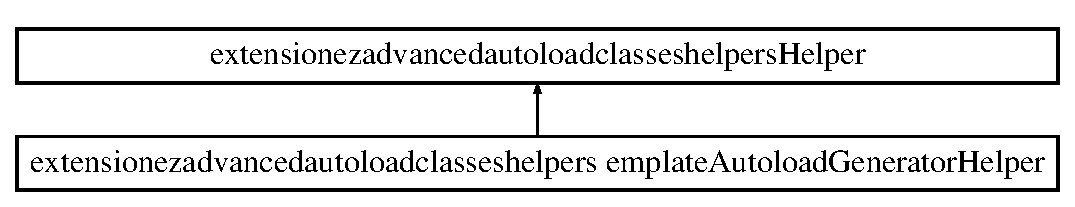
\includegraphics[height=2.000000cm]{classextension_1_1ezadvancedautoload_1_1classes_1_1helpers_1_1_helper}
\end{center}
\end{figure}
\subsection*{Public Member Functions}
\begin{DoxyCompactItemize}
\item 
\hyperlink{classextension_1_1ezadvancedautoload_1_1classes_1_1helpers_1_1_helper_add85e885141598709a72bfb9597faca7}{\-\_\-\-\_\-construct} ()
\begin{DoxyCompactList}\small\item\em There are no constructors for an abstract class. \end{DoxyCompactList}\item 
\hyperlink{classextension_1_1ezadvancedautoload_1_1classes_1_1helpers_1_1_helper_a1ba4093b3f040170370e36baaf970e60}{\-\_\-\-\_\-clone} ()
\begin{DoxyCompactList}\small\item\em An helper isn't clonable. \end{DoxyCompactList}\item 
\hyperlink{classextension_1_1ezadvancedautoload_1_1classes_1_1helpers_1_1_helper_a1bbf1edc42c8d0115a6164245faabf79}{\-\_\-\-\_\-sleep} ()
\begin{DoxyCompactList}\small\item\em An helper isn't serializable. \end{DoxyCompactList}\item 
\hyperlink{classextension_1_1ezadvancedautoload_1_1classes_1_1helpers_1_1_helper_a08df62000e6e73520c197c1f712e4ca8}{\-\_\-\-\_\-wakeup} ()
\begin{DoxyCompactList}\small\item\em An helper isn't serializable. \end{DoxyCompactList}\end{DoxyCompactItemize}


\subsection{Detailed Description}


Definition at line 17 of file helper.\-php.



\subsection{Constructor \& Destructor Documentation}
\hypertarget{classextension_1_1ezadvancedautoload_1_1classes_1_1helpers_1_1_helper_add85e885141598709a72bfb9597faca7}{\index{extension\-::ezadvancedautoload\-::classes\-::helpers\-::\-Helper@{extension\-::ezadvancedautoload\-::classes\-::helpers\-::\-Helper}!\-\_\-\-\_\-construct@{\-\_\-\-\_\-construct}}
\index{\-\_\-\-\_\-construct@{\-\_\-\-\_\-construct}!extension::ezadvancedautoload::classes::helpers::Helper@{extension\-::ezadvancedautoload\-::classes\-::helpers\-::\-Helper}}
\subsubsection[{\-\_\-\-\_\-construct}]{\setlength{\rightskip}{0pt plus 5cm}{\bf extension$\backslash$ezadvancedautoload$\backslash$classes$\backslash$helpers$\backslash$\-Helper\-::\-\_\-\-\_\-construct} (
\begin{DoxyParamCaption}
{}
\end{DoxyParamCaption}
)\hspace{0.3cm}{\ttfamily  \mbox{[}final\mbox{]}}}}\label{classextension_1_1ezadvancedautoload_1_1classes_1_1helpers_1_1_helper_add85e885141598709a72bfb9597faca7}


There are no constructors for an abstract class. 

There are no constructors for an abstract class

\begin{DoxyReturn}{Returns}
void 
\end{DoxyReturn}


Definition at line 25 of file helper.\-php.



\subsection{Member Function Documentation}
\hypertarget{classextension_1_1ezadvancedautoload_1_1classes_1_1helpers_1_1_helper_a1ba4093b3f040170370e36baaf970e60}{\index{extension\-::ezadvancedautoload\-::classes\-::helpers\-::\-Helper@{extension\-::ezadvancedautoload\-::classes\-::helpers\-::\-Helper}!\-\_\-\-\_\-clone@{\-\_\-\-\_\-clone}}
\index{\-\_\-\-\_\-clone@{\-\_\-\-\_\-clone}!extension::ezadvancedautoload::classes::helpers::Helper@{extension\-::ezadvancedautoload\-::classes\-::helpers\-::\-Helper}}
\subsubsection[{\-\_\-\-\_\-clone}]{\setlength{\rightskip}{0pt plus 5cm}{\bf extension$\backslash$ezadvancedautoload$\backslash$classes$\backslash$helpers$\backslash$\-Helper\-::\-\_\-\-\_\-clone} (
\begin{DoxyParamCaption}
{}
\end{DoxyParamCaption}
)\hspace{0.3cm}{\ttfamily  \mbox{[}final\mbox{]}}}}\label{classextension_1_1ezadvancedautoload_1_1classes_1_1helpers_1_1_helper_a1ba4093b3f040170370e36baaf970e60}


An helper isn't clonable. 

An helper isn't clonable

\begin{DoxyReturn}{Returns}
void 
\end{DoxyReturn}


Definition at line 35 of file helper.\-php.

\hypertarget{classextension_1_1ezadvancedautoload_1_1classes_1_1helpers_1_1_helper_a1bbf1edc42c8d0115a6164245faabf79}{\index{extension\-::ezadvancedautoload\-::classes\-::helpers\-::\-Helper@{extension\-::ezadvancedautoload\-::classes\-::helpers\-::\-Helper}!\-\_\-\-\_\-sleep@{\-\_\-\-\_\-sleep}}
\index{\-\_\-\-\_\-sleep@{\-\_\-\-\_\-sleep}!extension::ezadvancedautoload::classes::helpers::Helper@{extension\-::ezadvancedautoload\-::classes\-::helpers\-::\-Helper}}
\subsubsection[{\-\_\-\-\_\-sleep}]{\setlength{\rightskip}{0pt plus 5cm}{\bf extension$\backslash$ezadvancedautoload$\backslash$classes$\backslash$helpers$\backslash$\-Helper\-::\-\_\-\-\_\-sleep} (
\begin{DoxyParamCaption}
{}
\end{DoxyParamCaption}
)\hspace{0.3cm}{\ttfamily  \mbox{[}final\mbox{]}}}}\label{classextension_1_1ezadvancedautoload_1_1classes_1_1helpers_1_1_helper_a1bbf1edc42c8d0115a6164245faabf79}


An helper isn't serializable. 

An helper isn't serializable

\begin{DoxyReturn}{Returns}
void 
\end{DoxyReturn}


Definition at line 45 of file helper.\-php.

\hypertarget{classextension_1_1ezadvancedautoload_1_1classes_1_1helpers_1_1_helper_a08df62000e6e73520c197c1f712e4ca8}{\index{extension\-::ezadvancedautoload\-::classes\-::helpers\-::\-Helper@{extension\-::ezadvancedautoload\-::classes\-::helpers\-::\-Helper}!\-\_\-\-\_\-wakeup@{\-\_\-\-\_\-wakeup}}
\index{\-\_\-\-\_\-wakeup@{\-\_\-\-\_\-wakeup}!extension::ezadvancedautoload::classes::helpers::Helper@{extension\-::ezadvancedautoload\-::classes\-::helpers\-::\-Helper}}
\subsubsection[{\-\_\-\-\_\-wakeup}]{\setlength{\rightskip}{0pt plus 5cm}{\bf extension$\backslash$ezadvancedautoload$\backslash$classes$\backslash$helpers$\backslash$\-Helper\-::\-\_\-\-\_\-wakeup} (
\begin{DoxyParamCaption}
{}
\end{DoxyParamCaption}
)\hspace{0.3cm}{\ttfamily  \mbox{[}final\mbox{]}}}}\label{classextension_1_1ezadvancedautoload_1_1classes_1_1helpers_1_1_helper_a08df62000e6e73520c197c1f712e4ca8}


An helper isn't serializable. 

An helper isn't serializable

\begin{DoxyReturn}{Returns}
void 
\end{DoxyReturn}


Definition at line 55 of file helper.\-php.



The documentation for this class was generated from the following file\-:\begin{DoxyCompactItemize}
\item 
C\-:/\-Users/aloyant/ezadvancedautoload/classes/helpers/\hyperlink{helper_8php}{helper.\-php}\end{DoxyCompactItemize}

\hypertarget{classextension_1_1ezadvancedautoload_1_1classes_1_1helpers_1_1template_autoload_generator_helper}{\section{extension$\backslash$ezadvancedautoload$\backslash$classes$\backslash$helpers$\backslash$template\-Autoload\-Generator\-Helper \-Class \-Reference}
\label{classextension_1_1ezadvancedautoload_1_1classes_1_1helpers_1_1template_autoload_generator_helper}\index{extension$\backslash$ezadvancedautoload$\backslash$classes$\backslash$helpers$\backslash$template\-Autoload\-Generator\-Helper@{extension$\backslash$ezadvancedautoload$\backslash$classes$\backslash$helpers$\backslash$template\-Autoload\-Generator\-Helper}}
}
\-Inheritance diagram for extension$\backslash$ezadvancedautoload$\backslash$classes$\backslash$helpers$\backslash$template\-Autoload\-Generator\-Helper\-:\begin{figure}[H]
\begin{center}
\leavevmode
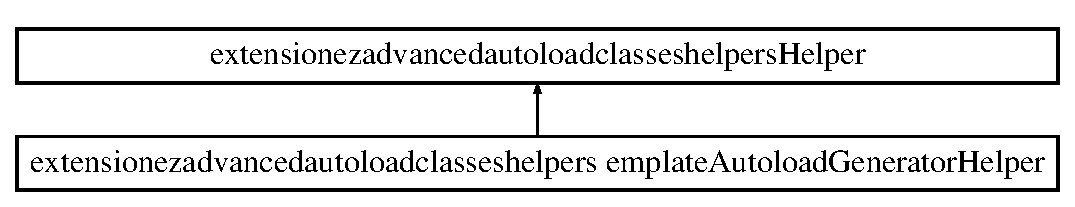
\includegraphics[height=2.000000cm]{classextension_1_1ezadvancedautoload_1_1classes_1_1helpers_1_1template_autoload_generator_helper}
\end{center}
\end{figure}
\subsection*{\-Static \-Public \-Member \-Functions}
\begin{DoxyCompactItemize}
\item 
static \hyperlink{classextension_1_1ezadvancedautoload_1_1classes_1_1helpers_1_1template_autoload_generator_helper_a9e7331253c8777a53e149cee0fec24e2}{regenerate} (\$mode,$\backslash$e\-Z\-Template \$template=null)
\item 
static \hyperlink{classextension_1_1ezadvancedautoload_1_1classes_1_1helpers_1_1template_autoload_generator_helper_a211ba9e5455710fff3650c6346bb25b2}{regenerate\-Kernel} ($\backslash$e\-Z\-Template \$template=null)
\begin{DoxyCompactList}\small\item\em \-Regenerate autoload for kernel only (ezp\-\_\-kernel) \end{DoxyCompactList}\item 
static \hyperlink{classextension_1_1ezadvancedautoload_1_1classes_1_1helpers_1_1template_autoload_generator_helper_a16974fee22eab241cc07d0cb204a1416}{regenerate\-Kernel\-Override} ($\backslash$e\-Z\-Template \$template=null)
\begin{DoxyCompactList}\small\item\em \-Regenerate autoload for kernel override only (ezp\-\_\-override) \end{DoxyCompactList}\item 
static \hyperlink{classextension_1_1ezadvancedautoload_1_1classes_1_1helpers_1_1template_autoload_generator_helper_a3d8b479039142fc9527828cc4e3e37b3}{regenerate\-Extension} ($\backslash$e\-Z\-Template \$template=null)
\begin{DoxyCompactList}\small\item\em \-Regenerate autoload for extension only (ezp\-\_\-extension) \end{DoxyCompactList}\item 
static \hyperlink{classextension_1_1ezadvancedautoload_1_1classes_1_1helpers_1_1template_autoload_generator_helper_a67ef43192f34d9f76711d37eeef46836}{regenerate\-Test} ($\backslash$e\-Z\-Template \$template=null)
\begin{DoxyCompactList}\small\item\em \-Regenerate autoload for tests only (ezp\-\_\-tests) \end{DoxyCompactList}\end{DoxyCompactItemize}
\subsection*{\-Static \-Private \-Member \-Functions}
\begin{DoxyCompactItemize}
\item 
static \hyperlink{classextension_1_1ezadvancedautoload_1_1classes_1_1helpers_1_1template_autoload_generator_helper_aa148374d28a61457d9e354c0d84df195}{run\-Generate} ($\backslash$ezp\-Autoload\-Generator\-Options \$autoload\-Options,$\backslash$e\-Z\-Template \$template=null)
\begin{DoxyCompactList}\small\item\em launch the regeneration \end{DoxyCompactList}\end{DoxyCompactItemize}


\subsection{\-Detailed \-Description}


\-Definition at line 21 of file templateautoloadgeneratorhelper.\-php.



\subsection{\-Member \-Function \-Documentation}
\hypertarget{classextension_1_1ezadvancedautoload_1_1classes_1_1helpers_1_1template_autoload_generator_helper_a9e7331253c8777a53e149cee0fec24e2}{\index{extension\-::ezadvancedautoload\-::classes\-::helpers\-::template\-Autoload\-Generator\-Helper@{extension\-::ezadvancedautoload\-::classes\-::helpers\-::template\-Autoload\-Generator\-Helper}!regenerate@{regenerate}}
\index{regenerate@{regenerate}!extension::ezadvancedautoload::classes::helpers::templateAutoloadGeneratorHelper@{extension\-::ezadvancedautoload\-::classes\-::helpers\-::template\-Autoload\-Generator\-Helper}}
\subsubsection[{regenerate}]{\setlength{\rightskip}{0pt plus 5cm}static extension$\backslash$ezadvancedautoload$\backslash$classes$\backslash$helpers$\backslash${\bf template\-Autoload\-Generator\-Helper\-::regenerate} (
\begin{DoxyParamCaption}
\item[{\$}]{mode, }
\item[{$\backslash$e\-Z\-Template \$}]{template = {\ttfamily null}}
\end{DoxyParamCaption}
)\hspace{0.3cm}{\ttfamily  \mbox{[}static\mbox{]}}}}\label{classextension_1_1ezadvancedautoload_1_1classes_1_1helpers_1_1template_autoload_generator_helper_a9e7331253c8777a53e149cee0fec24e2}


\-Definition at line 34 of file templateautoloadgeneratorhelper.\-php.



\-References extension$\backslash$ezadvancedautoload$\backslash$classes$\backslash$helpers$\backslash$template\-Autoload\-Generator\-Helper$\backslash$regenerate\-Extension(), extension$\backslash$ezadvancedautoload$\backslash$classes$\backslash$helpers$\backslash$template\-Autoload\-Generator\-Helper$\backslash$regenerate\-Kernel(), extension$\backslash$ezadvancedautoload$\backslash$classes$\backslash$helpers$\backslash$template\-Autoload\-Generator\-Helper$\backslash$regenerate\-Kernel\-Override(), and extension$\backslash$ezadvancedautoload$\backslash$classes$\backslash$helpers$\backslash$template\-Autoload\-Generator\-Helper$\backslash$regenerate\-Test().

\hypertarget{classextension_1_1ezadvancedautoload_1_1classes_1_1helpers_1_1template_autoload_generator_helper_a3d8b479039142fc9527828cc4e3e37b3}{\index{extension\-::ezadvancedautoload\-::classes\-::helpers\-::template\-Autoload\-Generator\-Helper@{extension\-::ezadvancedautoload\-::classes\-::helpers\-::template\-Autoload\-Generator\-Helper}!regenerate\-Extension@{regenerate\-Extension}}
\index{regenerate\-Extension@{regenerate\-Extension}!extension::ezadvancedautoload::classes::helpers::templateAutoloadGeneratorHelper@{extension\-::ezadvancedautoload\-::classes\-::helpers\-::template\-Autoload\-Generator\-Helper}}
\subsubsection[{regenerate\-Extension}]{\setlength{\rightskip}{0pt plus 5cm}static extension$\backslash$ezadvancedautoload$\backslash$classes$\backslash$helpers$\backslash${\bf template\-Autoload\-Generator\-Helper\-::regenerate\-Extension} (
\begin{DoxyParamCaption}
\item[{$\backslash$e\-Z\-Template \$}]{template = {\ttfamily null}}
\end{DoxyParamCaption}
)\hspace{0.3cm}{\ttfamily  \mbox{[}static\mbox{]}}}}\label{classextension_1_1ezadvancedautoload_1_1classes_1_1helpers_1_1template_autoload_generator_helper_a3d8b479039142fc9527828cc4e3e37b3}


\-Regenerate autoload for extension only (ezp\-\_\-extension) 

\-Regenerate autoload for extension only (ezp\-\_\-extension)


\begin{DoxyParams}{\-Parameters}
{\em $\backslash$e\-Z\-Template} & \$template the template to set the debug if we are in graphical mode \\
\hline
\end{DoxyParams}
\begin{DoxyReturn}{\-Returns}
void 
\end{DoxyReturn}


\-Definition at line 103 of file templateautoloadgeneratorhelper.\-php.



\-References \$autoload\-Options, and extension$\backslash$ezadvancedautoload$\backslash$classes$\backslash$helpers$\backslash$template\-Autoload\-Generator\-Helper$\backslash$run\-Generate().



\-Referenced by extension$\backslash$ezadvancedautoload$\backslash$classes$\backslash$helpers$\backslash$template\-Autoload\-Generator\-Helper$\backslash$regenerate().

\hypertarget{classextension_1_1ezadvancedautoload_1_1classes_1_1helpers_1_1template_autoload_generator_helper_a211ba9e5455710fff3650c6346bb25b2}{\index{extension\-::ezadvancedautoload\-::classes\-::helpers\-::template\-Autoload\-Generator\-Helper@{extension\-::ezadvancedautoload\-::classes\-::helpers\-::template\-Autoload\-Generator\-Helper}!regenerate\-Kernel@{regenerate\-Kernel}}
\index{regenerate\-Kernel@{regenerate\-Kernel}!extension::ezadvancedautoload::classes::helpers::templateAutoloadGeneratorHelper@{extension\-::ezadvancedautoload\-::classes\-::helpers\-::template\-Autoload\-Generator\-Helper}}
\subsubsection[{regenerate\-Kernel}]{\setlength{\rightskip}{0pt plus 5cm}static extension$\backslash$ezadvancedautoload$\backslash$classes$\backslash$helpers$\backslash${\bf template\-Autoload\-Generator\-Helper\-::regenerate\-Kernel} (
\begin{DoxyParamCaption}
\item[{$\backslash$e\-Z\-Template \$}]{template = {\ttfamily null}}
\end{DoxyParamCaption}
)\hspace{0.3cm}{\ttfamily  \mbox{[}static\mbox{]}}}}\label{classextension_1_1ezadvancedautoload_1_1classes_1_1helpers_1_1template_autoload_generator_helper_a211ba9e5455710fff3650c6346bb25b2}


\-Regenerate autoload for kernel only (ezp\-\_\-kernel) 

\-Regenerate autoload for kernel only (ezp\-\_\-kernel)


\begin{DoxyParams}{\-Parameters}
{\em $\backslash$e\-Z\-Template} & \$template the template to set the debug if we are in graphical mode \\
\hline
\end{DoxyParams}
\begin{DoxyReturn}{\-Returns}
void 
\end{DoxyReturn}


\-Definition at line 69 of file templateautoloadgeneratorhelper.\-php.



\-References \$autoload\-Options, and extension$\backslash$ezadvancedautoload$\backslash$classes$\backslash$helpers$\backslash$template\-Autoload\-Generator\-Helper$\backslash$run\-Generate().



\-Referenced by extension$\backslash$ezadvancedautoload$\backslash$classes$\backslash$helpers$\backslash$template\-Autoload\-Generator\-Helper$\backslash$regenerate().

\hypertarget{classextension_1_1ezadvancedautoload_1_1classes_1_1helpers_1_1template_autoload_generator_helper_a16974fee22eab241cc07d0cb204a1416}{\index{extension\-::ezadvancedautoload\-::classes\-::helpers\-::template\-Autoload\-Generator\-Helper@{extension\-::ezadvancedautoload\-::classes\-::helpers\-::template\-Autoload\-Generator\-Helper}!regenerate\-Kernel\-Override@{regenerate\-Kernel\-Override}}
\index{regenerate\-Kernel\-Override@{regenerate\-Kernel\-Override}!extension::ezadvancedautoload::classes::helpers::templateAutoloadGeneratorHelper@{extension\-::ezadvancedautoload\-::classes\-::helpers\-::template\-Autoload\-Generator\-Helper}}
\subsubsection[{regenerate\-Kernel\-Override}]{\setlength{\rightskip}{0pt plus 5cm}static extension$\backslash$ezadvancedautoload$\backslash$classes$\backslash$helpers$\backslash${\bf template\-Autoload\-Generator\-Helper\-::regenerate\-Kernel\-Override} (
\begin{DoxyParamCaption}
\item[{$\backslash$e\-Z\-Template \$}]{template = {\ttfamily null}}
\end{DoxyParamCaption}
)\hspace{0.3cm}{\ttfamily  \mbox{[}static\mbox{]}}}}\label{classextension_1_1ezadvancedautoload_1_1classes_1_1helpers_1_1template_autoload_generator_helper_a16974fee22eab241cc07d0cb204a1416}


\-Regenerate autoload for kernel override only (ezp\-\_\-override) 

\-Regenerate autoload for kernel override only (ezp\-\_\-override)


\begin{DoxyParams}{\-Parameters}
{\em $\backslash$e\-Z\-Template} & \$template the template to set the debug if we are in graphical mode \\
\hline
\end{DoxyParams}
\begin{DoxyReturn}{\-Returns}
void 
\end{DoxyReturn}


\-Definition at line 86 of file templateautoloadgeneratorhelper.\-php.



\-References \$autoload\-Options, and extension$\backslash$ezadvancedautoload$\backslash$classes$\backslash$helpers$\backslash$template\-Autoload\-Generator\-Helper$\backslash$run\-Generate().



\-Referenced by extension$\backslash$ezadvancedautoload$\backslash$classes$\backslash$helpers$\backslash$template\-Autoload\-Generator\-Helper$\backslash$regenerate().

\hypertarget{classextension_1_1ezadvancedautoload_1_1classes_1_1helpers_1_1template_autoload_generator_helper_a67ef43192f34d9f76711d37eeef46836}{\index{extension\-::ezadvancedautoload\-::classes\-::helpers\-::template\-Autoload\-Generator\-Helper@{extension\-::ezadvancedautoload\-::classes\-::helpers\-::template\-Autoload\-Generator\-Helper}!regenerate\-Test@{regenerate\-Test}}
\index{regenerate\-Test@{regenerate\-Test}!extension::ezadvancedautoload::classes::helpers::templateAutoloadGeneratorHelper@{extension\-::ezadvancedautoload\-::classes\-::helpers\-::template\-Autoload\-Generator\-Helper}}
\subsubsection[{regenerate\-Test}]{\setlength{\rightskip}{0pt plus 5cm}static extension$\backslash$ezadvancedautoload$\backslash$classes$\backslash$helpers$\backslash${\bf template\-Autoload\-Generator\-Helper\-::regenerate\-Test} (
\begin{DoxyParamCaption}
\item[{$\backslash$e\-Z\-Template \$}]{template = {\ttfamily null}}
\end{DoxyParamCaption}
)\hspace{0.3cm}{\ttfamily  \mbox{[}static\mbox{]}}}}\label{classextension_1_1ezadvancedautoload_1_1classes_1_1helpers_1_1template_autoload_generator_helper_a67ef43192f34d9f76711d37eeef46836}


\-Regenerate autoload for tests only (ezp\-\_\-tests) 

\-Regenerate autoload for tests only (ezp\-\_\-tests)


\begin{DoxyParams}{\-Parameters}
{\em $\backslash$e\-Z\-Template} & \$template the template to set the debug if we are in graphical mode \\
\hline
\end{DoxyParams}
\begin{DoxyReturn}{\-Returns}
void 
\end{DoxyReturn}


\-Definition at line 120 of file templateautoloadgeneratorhelper.\-php.



\-References \$autoload\-Options, and extension$\backslash$ezadvancedautoload$\backslash$classes$\backslash$helpers$\backslash$template\-Autoload\-Generator\-Helper$\backslash$run\-Generate().



\-Referenced by extension$\backslash$ezadvancedautoload$\backslash$classes$\backslash$helpers$\backslash$template\-Autoload\-Generator\-Helper$\backslash$regenerate().

\hypertarget{classextension_1_1ezadvancedautoload_1_1classes_1_1helpers_1_1template_autoload_generator_helper_aa148374d28a61457d9e354c0d84df195}{\index{extension\-::ezadvancedautoload\-::classes\-::helpers\-::template\-Autoload\-Generator\-Helper@{extension\-::ezadvancedautoload\-::classes\-::helpers\-::template\-Autoload\-Generator\-Helper}!run\-Generate@{run\-Generate}}
\index{run\-Generate@{run\-Generate}!extension::ezadvancedautoload::classes::helpers::templateAutoloadGeneratorHelper@{extension\-::ezadvancedautoload\-::classes\-::helpers\-::template\-Autoload\-Generator\-Helper}}
\subsubsection[{run\-Generate}]{\setlength{\rightskip}{0pt plus 5cm}static extension$\backslash$ezadvancedautoload$\backslash$classes$\backslash$helpers$\backslash${\bf template\-Autoload\-Generator\-Helper\-::run\-Generate} (
\begin{DoxyParamCaption}
\item[{$\backslash$ezp\-Autoload\-Generator\-Options \$}]{autoload\-Options, }
\item[{$\backslash$e\-Z\-Template \$}]{template = {\ttfamily null}}
\end{DoxyParamCaption}
)\hspace{0.3cm}{\ttfamily  \mbox{[}static, private\mbox{]}}}}\label{classextension_1_1ezadvancedautoload_1_1classes_1_1helpers_1_1template_autoload_generator_helper_aa148374d28a61457d9e354c0d84df195}


launch the regeneration 

launch the regeneration


\begin{DoxyParams}{\-Parameters}
{\em $\backslash$ezp\-Autoload\-Generator\-Options} & \$autoload\-Options the options to generate autoload \\
\hline
{\em $\backslash$e\-Z\-Template} & \$template the template to set the debug if we are in graphical mode \\
\hline
\end{DoxyParams}
\begin{DoxyReturn}{\-Returns}
void 
\end{DoxyReturn}


\-Definition at line 138 of file templateautoloadgeneratorhelper.\-php.



\-References \$autoload\-Generator.



\-Referenced by extension$\backslash$ezadvancedautoload$\backslash$classes$\backslash$helpers$\backslash$template\-Autoload\-Generator\-Helper$\backslash$regenerate\-Extension(), extension$\backslash$ezadvancedautoload$\backslash$classes$\backslash$helpers$\backslash$template\-Autoload\-Generator\-Helper$\backslash$regenerate\-Kernel(), extension$\backslash$ezadvancedautoload$\backslash$classes$\backslash$helpers$\backslash$template\-Autoload\-Generator\-Helper$\backslash$regenerate\-Kernel\-Override(), and extension$\backslash$ezadvancedautoload$\backslash$classes$\backslash$helpers$\backslash$template\-Autoload\-Generator\-Helper$\backslash$regenerate\-Test().



\-The documentation for this class was generated from the following file\-:\begin{DoxyCompactItemize}
\item 
\-D\-:/git/ezadvancedautoload/classes/helpers/\hyperlink{templateautoloadgeneratorhelper_8php}{templateautoloadgeneratorhelper.\-php}\end{DoxyCompactItemize}

\hypertarget{classextension_1_1ezadvancedautoload_1_1classes_1_1exceptions_1_1unexpected_mode_exception}{\section{extension$\backslash$ezadvancedautoload$\backslash$classes$\backslash$exceptions$\backslash$unexpected\-Mode\-Exception \-Class \-Reference}
\label{classextension_1_1ezadvancedautoload_1_1classes_1_1exceptions_1_1unexpected_mode_exception}\index{extension$\backslash$ezadvancedautoload$\backslash$classes$\backslash$exceptions$\backslash$unexpected\-Mode\-Exception@{extension$\backslash$ezadvancedautoload$\backslash$classes$\backslash$exceptions$\backslash$unexpected\-Mode\-Exception}}
}
\subsection*{\-Public \-Member \-Functions}
\begin{DoxyCompactItemize}
\item 
\hyperlink{classextension_1_1ezadvancedautoload_1_1classes_1_1exceptions_1_1unexpected_mode_exception_a487408899c0e62f331bc4942200fbaa3}{\-\_\-\-\_\-construct} (\$mode=null, \$code=null,$\backslash$\-Exception \$previous=null)
\begin{DoxyCompactList}\small\item\em \hyperlink{classextension_1_1ezadvancedautoload_1_1classes_1_1exceptions_1_1unexpected_mode_exception}{unexpected\-Mode\-Exception} constructor \end{DoxyCompactList}\end{DoxyCompactItemize}
\subsection*{\-Private \-Attributes}
\begin{DoxyCompactItemize}
\item 
\hyperlink{classextension_1_1ezadvancedautoload_1_1classes_1_1exceptions_1_1unexpected_mode_exception_a33b449881502e0ea0461e98b4fe47837}{\$mode}
\end{DoxyCompactItemize}


\subsection{\-Detailed \-Description}


\-Definition at line 17 of file unexpectedmodeexception.\-php.



\subsection{\-Constructor \& \-Destructor \-Documentation}
\hypertarget{classextension_1_1ezadvancedautoload_1_1classes_1_1exceptions_1_1unexpected_mode_exception_a487408899c0e62f331bc4942200fbaa3}{\index{extension\-::ezadvancedautoload\-::classes\-::exceptions\-::unexpected\-Mode\-Exception@{extension\-::ezadvancedautoload\-::classes\-::exceptions\-::unexpected\-Mode\-Exception}!\-\_\-\-\_\-construct@{\-\_\-\-\_\-construct}}
\index{\-\_\-\-\_\-construct@{\-\_\-\-\_\-construct}!extension::ezadvancedautoload::classes::exceptions::unexpectedModeException@{extension\-::ezadvancedautoload\-::classes\-::exceptions\-::unexpected\-Mode\-Exception}}
\subsubsection[{\-\_\-\-\_\-construct}]{\setlength{\rightskip}{0pt plus 5cm}extension$\backslash$ezadvancedautoload$\backslash$classes$\backslash$exceptions$\backslash${\bf unexpected\-Mode\-Exception\-::\-\_\-\-\_\-construct} (
\begin{DoxyParamCaption}
\item[{\$}]{mode = {\ttfamily null}, }
\item[{\$}]{code = {\ttfamily null}, }
\item[{$\backslash$\-Exception \$}]{previous = {\ttfamily null}}
\end{DoxyParamCaption}
)}}\label{classextension_1_1ezadvancedautoload_1_1classes_1_1exceptions_1_1unexpected_mode_exception_a487408899c0e62f331bc4942200fbaa3}


\hyperlink{classextension_1_1ezadvancedautoload_1_1classes_1_1exceptions_1_1unexpected_mode_exception}{unexpected\-Mode\-Exception} constructor 

\hyperlink{classextension_1_1ezadvancedautoload_1_1classes_1_1exceptions_1_1unexpected_mode_exception}{unexpected\-Mode\-Exception} constructor


\begin{DoxyParams}[1]{\-Parameters}
int & {\em \$mode} & \\
\hline
int & {\em \$code} & \\
\hline
 & {\em $\backslash$\-Exception} & \$previous \\
\hline
\end{DoxyParams}


\-Definition at line 35 of file unexpectedmodeexception.\-php.



\-References extension$\backslash$ezadvancedautoload$\backslash$classes$\backslash$exceptions$\backslash$unexpected\-Mode\-Exception$\backslash$\$mode.



\subsection{\-Member \-Data \-Documentation}
\hypertarget{classextension_1_1ezadvancedautoload_1_1classes_1_1exceptions_1_1unexpected_mode_exception_a33b449881502e0ea0461e98b4fe47837}{\index{extension\-::ezadvancedautoload\-::classes\-::exceptions\-::unexpected\-Mode\-Exception@{extension\-::ezadvancedautoload\-::classes\-::exceptions\-::unexpected\-Mode\-Exception}!\$mode@{\$mode}}
\index{\$mode@{\$mode}!extension::ezadvancedautoload::classes::exceptions::unexpectedModeException@{extension\-::ezadvancedautoload\-::classes\-::exceptions\-::unexpected\-Mode\-Exception}}
\subsubsection[{\$mode}]{\setlength{\rightskip}{0pt plus 5cm}extension\-::ezadvancedautoload\-::classes\-::exceptions$\backslash$unexpected\-Mode\-Exception\-::\$mode\hspace{0.3cm}{\ttfamily  \mbox{[}private\mbox{]}}}}\label{classextension_1_1ezadvancedautoload_1_1classes_1_1exceptions_1_1unexpected_mode_exception_a33b449881502e0ea0461e98b4fe47837}


\-Definition at line 25 of file unexpectedmodeexception.\-php.



\-Referenced by extension$\backslash$ezadvancedautoload$\backslash$classes$\backslash$exceptions$\backslash$unexpected\-Mode\-Exception$\backslash$\-\_\-\-\_\-construct().



\-The documentation for this class was generated from the following file\-:\begin{DoxyCompactItemize}
\item 
\-D\-:/git/ezadvancedautoload/classes/exceptions/\hyperlink{unexpectedmodeexception_8php}{unexpectedmodeexception.\-php}\end{DoxyCompactItemize}

\chapter{File Documentation}
\hypertarget{ezpgenerateautoloads_8php}{\section{C\-:/\-Users/aloyant/ezadvancedautoload/bin/php/ezpgenerateautoloads.php File Reference}
\label{ezpgenerateautoloads_8php}\index{C\-:/\-Users/aloyant/ezadvancedautoload/bin/php/ezpgenerateautoloads.\-php@{C\-:/\-Users/aloyant/ezadvancedautoload/bin/php/ezpgenerateautoloads.\-php}}
}
\subsection*{Variables}
\begin{DoxyCompactItemize}
\item 
if(file\-\_\-exists('config.\-php')) \hyperlink{ezpgenerateautoloads_8php_abdb1c04b56bd870d8c95d438c1a3ceb7}{\$use\-Bundled\-Components} = defined( 'E\-Z\-P\-\_\-\-U\-S\-E\-\_\-\-B\-U\-N\-D\-L\-E\-D\-\_\-\-C\-O\-M\-P\-O\-N\-E\-N\-T\-S' ) ? E\-Z\-P\-\_\-\-U\-S\-E\-\_\-\-B\-U\-N\-D\-L\-E\-D\-\_\-\-C\-O\-M\-P\-O\-N\-E\-N\-T\-S === true \-: file\-\_\-exists( 'lib/ezc' )
\item 
\hyperlink{ezpgenerateautoloads_8php_afe68e6fbe7acfbffc0af0c84a1996466}{\$params} = new ezc\-Console\-Input()
\item 
\hyperlink{ezpgenerateautoloads_8php_a785ce4531ef75b21040c99c8cbce7aa4}{\$help\-Option} = new ezc\-Console\-Option( 'h', 'help' )
\item 
\$help\-Option \hyperlink{ezpgenerateautoloads_8php_ac38115d855b4d48735ec865ab62bf1fe}{mandatory} = false
\item 
\$help\-Option \hyperlink{ezpgenerateautoloads_8php_a6878132bff242d248a03a92df0ead036}{shorthelp} = 'Show help information'
\item 
\hyperlink{ezpgenerateautoloads_8php_a6b7b596c6eccab7f3c39bbcad2d711a0}{\$target\-Option} = new ezc\-Console\-Option( 't', 'target', ezc\-Console\-Input\-::\-T\-Y\-P\-E\-\_\-\-S\-T\-R\-I\-N\-G )
\item 
\hyperlink{ezpgenerateautoloads_8php_a22133d0c8998aa2d18623686cca5faa4}{\$verbose\-Option} = new ezc\-Console\-Option( 'v', 'verbose', ezc\-Console\-Input\-::\-T\-Y\-P\-E\-\_\-\-N\-O\-N\-E )
\item 
\hyperlink{ezpgenerateautoloads_8php_a2157a552be64e9a75918a23fef9e26e7}{\$dryrun\-Option} = new ezc\-Console\-Option( 'n', 'dry-\/run', ezc\-Console\-Input\-::\-T\-Y\-P\-E\-\_\-\-N\-O\-N\-E )
\item 
\hyperlink{ezpgenerateautoloads_8php_a7e74e8adf0bd544754962f4ddd4fc35b}{\$kernel\-Files\-Option} = new ezc\-Console\-Option( 'k', 'kernel', ezc\-Console\-Input\-::\-T\-Y\-P\-E\-\_\-\-N\-O\-N\-E )
\item 
\hyperlink{ezpgenerateautoloads_8php_a67e31a42e7cb071e5c02df2261d6594a}{\$kernel\-Override\-Option} = new ezc\-Console\-Option( 'o', 'kernel-\/override', ezc\-Console\-Input\-::\-T\-Y\-P\-E\-\_\-\-N\-O\-N\-E )
\item 
\hyperlink{ezpgenerateautoloads_8php_a35b967cec5da82cfa9989e036ad50642}{\$extension\-Files\-Option} = new ezc\-Console\-Option( 'e', 'extension', ezc\-Console\-Input\-::\-T\-Y\-P\-E\-\_\-\-N\-O\-N\-E )
\item 
\hyperlink{ezpgenerateautoloads_8php_a42bc54b597a301809a0bdbec1c8f1ee6}{\$test\-Files\-Option} = new ezc\-Console\-Option( 's', 'tests', ezc\-Console\-Input\-::\-T\-Y\-P\-E\-\_\-\-N\-O\-N\-E )
\item 
\hyperlink{ezpgenerateautoloads_8php_ad444c7af1932b7a85e8351702c783790}{\$exclude\-Dirs\-Option} = new ezc\-Console\-Option( '', 'exclude', ezc\-Console\-Input\-::\-T\-Y\-P\-E\-\_\-\-S\-T\-R\-I\-N\-G )
\item 
\hyperlink{ezpgenerateautoloads_8php_a407bf0b4ef42d32212f29ac7c8e8a96e}{\$display\-Progress\-Option} = new ezc\-Console\-Option( 'p', 'progress', ezc\-Console\-Input\-::\-T\-Y\-P\-E\-\_\-\-N\-O\-N\-E )
\item 
\$params \hyperlink{ezpgenerateautoloads_8php_ab9a0a1710f335bc48a13e8a94802be23}{argument\-Definition} = new ezc\-Console\-Arguments()
\item 
\$params \hyperlink{ezpgenerateautoloads_8php_aed0ba19f5204d9659e823271642a6594}{argument\-Definition} \mbox{[}0\mbox{]} = new ezc\-Console\-Argument( 'extension' )
\item 
\$params \hyperlink{ezpgenerateautoloads_8php_aed0ba19f5204d9659e823271642a6594}{argument\-Definition}\mbox{[}0\mbox{]} \hyperlink{ezpgenerateautoloads_8php_a7cbde127000429b4c1ee76be227eca44}{default} = getcwd()
\item 
if(\$exclude\-Dirs\-Option-\/$>$value!==false) \hyperlink{ezpgenerateautoloads_8php_a11b2b8d92ed8fe93c2e53197e661142c}{\$autoload\-Options} = new ezp\-Autoload\-Generator\-Options()
\item 
\$autoload\-Options \hyperlink{ezpgenerateautoloads_8php_a29816a8455ff45c83cd2e389735c8207}{base\-Path} = \$params-\/$>$\hyperlink{ezpgenerateautoloads_8php_aed0ba19f5204d9659e823271642a6594}{argument\-Definition}\mbox{[}'extension'\mbox{]}-\/$>$value
\item 
\$autoload\-Options \hyperlink{ezpgenerateautoloads_8php_aab46cc9fff71273094aafac8ebd689d4}{search\-Kernel\-Files} = \$kernel\-Files\-Option-\/$>$value
\item 
\$autoload\-Options \hyperlink{ezpgenerateautoloads_8php_af86b9a19664645803f32b4d5bb872ff1}{search\-Kernel\-Override} = \$kernel\-Override\-Option-\/$>$value
\item 
\$autoload\-Options \hyperlink{ezpgenerateautoloads_8php_ae648f5335e57fa264ffaaf9d2fe4c61b}{search\-Extension\-Files} = \$extension\-Files\-Option-\/$>$value
\item 
\$autoload\-Options \hyperlink{ezpgenerateautoloads_8php_a3727c480754aa7c8b3dc7e8070ed1eb4}{search\-Test\-Files} = \$test\-Files\-Option-\/$>$value
\item 
\$autoload\-Options \hyperlink{ezpgenerateautoloads_8php_a210f8683b204a76199152312e3d9a177}{write\-Files} = !\$dryrun\-Option-\/$>$value
\item 
\$autoload\-Options \hyperlink{ezpgenerateautoloads_8php_aa79f55582aba2bd3eff4d3fa4b980a84}{display\-Progress} = \$display\-Progress\-Option-\/$>$value
\item 
if(!empty(\$target\-Option-\/$>$value)) \\*
\$autoload\-Options \hyperlink{ezpgenerateautoloads_8php_a52217447e9aa7d329a16ea69370b42a4}{exclude\-Dirs} = \$\hyperlink{ezpgenerateautoloads_8php_a52217447e9aa7d329a16ea69370b42a4}{exclude\-Dirs}
\item 
\hyperlink{ezpgenerateautoloads_8php_a86e95d193d321273aadaef08750683a8}{\$autoload\-Generator} = new $\backslash$extension$\backslash$ezadvancedautoload$\backslash$e\-Z\-Autoload\-Generator( \$autoload\-Options )
\end{DoxyCompactItemize}


\subsection{Variable Documentation}
\hypertarget{ezpgenerateautoloads_8php_a86e95d193d321273aadaef08750683a8}{\index{ezpgenerateautoloads.\-php@{ezpgenerateautoloads.\-php}!\$autoload\-Generator@{\$autoload\-Generator}}
\index{\$autoload\-Generator@{\$autoload\-Generator}!ezpgenerateautoloads.php@{ezpgenerateautoloads.\-php}}
\subsubsection[{\$autoload\-Generator}]{\setlength{\rightskip}{0pt plus 5cm}\$autoload\-Generator = new $\backslash$extension$\backslash$ezadvancedautoload$\backslash$e\-Z\-Autoload\-Generator( \$autoload\-Options )}}\label{ezpgenerateautoloads_8php_a86e95d193d321273aadaef08750683a8}


Definition at line 153 of file ezpgenerateautoloads.\-php.



Referenced by extension$\backslash$ezadvancedautoload$\backslash$classes$\backslash$helpers$\backslash$template\-Autoload\-Generator\-Helper$\backslash$run\-Generate().

\hypertarget{ezpgenerateautoloads_8php_a11b2b8d92ed8fe93c2e53197e661142c}{\index{ezpgenerateautoloads.\-php@{ezpgenerateautoloads.\-php}!\$autoload\-Options@{\$autoload\-Options}}
\index{\$autoload\-Options@{\$autoload\-Options}!ezpgenerateautoloads.php@{ezpgenerateautoloads.\-php}}
\subsubsection[{\$autoload\-Options}]{\setlength{\rightskip}{0pt plus 5cm}if (\$exclude\-Dirs\-Option-\/$>$value!==false) \$autoload\-Options = new ezp\-Autoload\-Generator\-Options()}}\label{ezpgenerateautoloads_8php_a11b2b8d92ed8fe93c2e53197e661142c}


Definition at line 137 of file ezpgenerateautoloads.\-php.



Referenced by extension$\backslash$ezadvancedautoload$\backslash$classes$\backslash$helpers$\backslash$template\-Autoload\-Generator\-Helper$\backslash$regenerate\-Extension(), extension$\backslash$ezadvancedautoload$\backslash$classes$\backslash$helpers$\backslash$template\-Autoload\-Generator\-Helper$\backslash$regenerate\-Kernel(), extension$\backslash$ezadvancedautoload$\backslash$classes$\backslash$helpers$\backslash$template\-Autoload\-Generator\-Helper$\backslash$regenerate\-Kernel\-Override(), and extension$\backslash$ezadvancedautoload$\backslash$classes$\backslash$helpers$\backslash$template\-Autoload\-Generator\-Helper$\backslash$regenerate\-Test().

\hypertarget{ezpgenerateautoloads_8php_a407bf0b4ef42d32212f29ac7c8e8a96e}{\index{ezpgenerateautoloads.\-php@{ezpgenerateautoloads.\-php}!\$display\-Progress\-Option@{\$display\-Progress\-Option}}
\index{\$display\-Progress\-Option@{\$display\-Progress\-Option}!ezpgenerateautoloads.php@{ezpgenerateautoloads.\-php}}
\subsubsection[{\$display\-Progress\-Option}]{\setlength{\rightskip}{0pt plus 5cm}\$display\-Progress\-Option = new ezc\-Console\-Option( 'p', 'progress', ezc\-Console\-Input\-::\-T\-Y\-P\-E\-\_\-\-N\-O\-N\-E )}}\label{ezpgenerateautoloads_8php_a407bf0b4ef42d32212f29ac7c8e8a96e}


Definition at line 99 of file ezpgenerateautoloads.\-php.

\hypertarget{ezpgenerateautoloads_8php_a2157a552be64e9a75918a23fef9e26e7}{\index{ezpgenerateautoloads.\-php@{ezpgenerateautoloads.\-php}!\$dryrun\-Option@{\$dryrun\-Option}}
\index{\$dryrun\-Option@{\$dryrun\-Option}!ezpgenerateautoloads.php@{ezpgenerateautoloads.\-php}}
\subsubsection[{\$dryrun\-Option}]{\setlength{\rightskip}{0pt plus 5cm}\$dryrun\-Option = new ezc\-Console\-Option( 'n', 'dry-\/run', ezc\-Console\-Input\-::\-T\-Y\-P\-E\-\_\-\-N\-O\-N\-E )}}\label{ezpgenerateautoloads_8php_a2157a552be64e9a75918a23fef9e26e7}


Definition at line 69 of file ezpgenerateautoloads.\-php.

\hypertarget{ezpgenerateautoloads_8php_ad444c7af1932b7a85e8351702c783790}{\index{ezpgenerateautoloads.\-php@{ezpgenerateautoloads.\-php}!\$exclude\-Dirs\-Option@{\$exclude\-Dirs\-Option}}
\index{\$exclude\-Dirs\-Option@{\$exclude\-Dirs\-Option}!ezpgenerateautoloads.php@{ezpgenerateautoloads.\-php}}
\subsubsection[{\$exclude\-Dirs\-Option}]{\setlength{\rightskip}{0pt plus 5cm}\$exclude\-Dirs\-Option = new ezc\-Console\-Option( '', 'exclude', ezc\-Console\-Input\-::\-T\-Y\-P\-E\-\_\-\-S\-T\-R\-I\-N\-G )}}\label{ezpgenerateautoloads_8php_ad444c7af1932b7a85e8351702c783790}


Definition at line 94 of file ezpgenerateautoloads.\-php.

\hypertarget{ezpgenerateautoloads_8php_a35b967cec5da82cfa9989e036ad50642}{\index{ezpgenerateautoloads.\-php@{ezpgenerateautoloads.\-php}!\$extension\-Files\-Option@{\$extension\-Files\-Option}}
\index{\$extension\-Files\-Option@{\$extension\-Files\-Option}!ezpgenerateautoloads.php@{ezpgenerateautoloads.\-php}}
\subsubsection[{\$extension\-Files\-Option}]{\setlength{\rightskip}{0pt plus 5cm}\$extension\-Files\-Option = new ezc\-Console\-Option( 'e', 'extension', ezc\-Console\-Input\-::\-T\-Y\-P\-E\-\_\-\-N\-O\-N\-E )}}\label{ezpgenerateautoloads_8php_a35b967cec5da82cfa9989e036ad50642}


Definition at line 84 of file ezpgenerateautoloads.\-php.

\hypertarget{ezpgenerateautoloads_8php_a785ce4531ef75b21040c99c8cbce7aa4}{\index{ezpgenerateautoloads.\-php@{ezpgenerateautoloads.\-php}!\$help\-Option@{\$help\-Option}}
\index{\$help\-Option@{\$help\-Option}!ezpgenerateautoloads.php@{ezpgenerateautoloads.\-php}}
\subsubsection[{\$help\-Option}]{\setlength{\rightskip}{0pt plus 5cm}\$help\-Option = new ezc\-Console\-Option( 'h', 'help' )}}\label{ezpgenerateautoloads_8php_a785ce4531ef75b21040c99c8cbce7aa4}


Definition at line 54 of file ezpgenerateautoloads.\-php.

\hypertarget{ezpgenerateautoloads_8php_a7e74e8adf0bd544754962f4ddd4fc35b}{\index{ezpgenerateautoloads.\-php@{ezpgenerateautoloads.\-php}!\$kernel\-Files\-Option@{\$kernel\-Files\-Option}}
\index{\$kernel\-Files\-Option@{\$kernel\-Files\-Option}!ezpgenerateautoloads.php@{ezpgenerateautoloads.\-php}}
\subsubsection[{\$kernel\-Files\-Option}]{\setlength{\rightskip}{0pt plus 5cm}\$kernel\-Files\-Option = new ezc\-Console\-Option( 'k', 'kernel', ezc\-Console\-Input\-::\-T\-Y\-P\-E\-\_\-\-N\-O\-N\-E )}}\label{ezpgenerateautoloads_8php_a7e74e8adf0bd544754962f4ddd4fc35b}


Definition at line 74 of file ezpgenerateautoloads.\-php.

\hypertarget{ezpgenerateautoloads_8php_a67e31a42e7cb071e5c02df2261d6594a}{\index{ezpgenerateautoloads.\-php@{ezpgenerateautoloads.\-php}!\$kernel\-Override\-Option@{\$kernel\-Override\-Option}}
\index{\$kernel\-Override\-Option@{\$kernel\-Override\-Option}!ezpgenerateautoloads.php@{ezpgenerateautoloads.\-php}}
\subsubsection[{\$kernel\-Override\-Option}]{\setlength{\rightskip}{0pt plus 5cm}\$kernel\-Override\-Option = new ezc\-Console\-Option( 'o', 'kernel-\/override', ezc\-Console\-Input\-::\-T\-Y\-P\-E\-\_\-\-N\-O\-N\-E )}}\label{ezpgenerateautoloads_8php_a67e31a42e7cb071e5c02df2261d6594a}


Definition at line 79 of file ezpgenerateautoloads.\-php.

\hypertarget{ezpgenerateautoloads_8php_afe68e6fbe7acfbffc0af0c84a1996466}{\index{ezpgenerateautoloads.\-php@{ezpgenerateautoloads.\-php}!\$params@{\$params}}
\index{\$params@{\$params}!ezpgenerateautoloads.php@{ezpgenerateautoloads.\-php}}
\subsubsection[{\$params}]{\setlength{\rightskip}{0pt plus 5cm}\$params = new ezc\-Console\-Input()}}\label{ezpgenerateautoloads_8php_afe68e6fbe7acfbffc0af0c84a1996466}


Definition at line 52 of file ezpgenerateautoloads.\-php.

\hypertarget{ezpgenerateautoloads_8php_a6b7b596c6eccab7f3c39bbcad2d711a0}{\index{ezpgenerateautoloads.\-php@{ezpgenerateautoloads.\-php}!\$target\-Option@{\$target\-Option}}
\index{\$target\-Option@{\$target\-Option}!ezpgenerateautoloads.php@{ezpgenerateautoloads.\-php}}
\subsubsection[{\$target\-Option}]{\setlength{\rightskip}{0pt plus 5cm}\$target\-Option = new ezc\-Console\-Option( 't', 'target', ezc\-Console\-Input\-::\-T\-Y\-P\-E\-\_\-\-S\-T\-R\-I\-N\-G )}}\label{ezpgenerateautoloads_8php_a6b7b596c6eccab7f3c39bbcad2d711a0}


Definition at line 59 of file ezpgenerateautoloads.\-php.

\hypertarget{ezpgenerateautoloads_8php_a42bc54b597a301809a0bdbec1c8f1ee6}{\index{ezpgenerateautoloads.\-php@{ezpgenerateautoloads.\-php}!\$test\-Files\-Option@{\$test\-Files\-Option}}
\index{\$test\-Files\-Option@{\$test\-Files\-Option}!ezpgenerateautoloads.php@{ezpgenerateautoloads.\-php}}
\subsubsection[{\$test\-Files\-Option}]{\setlength{\rightskip}{0pt plus 5cm}\$test\-Files\-Option = new ezc\-Console\-Option( 's', 'tests', ezc\-Console\-Input\-::\-T\-Y\-P\-E\-\_\-\-N\-O\-N\-E )}}\label{ezpgenerateautoloads_8php_a42bc54b597a301809a0bdbec1c8f1ee6}


Definition at line 89 of file ezpgenerateautoloads.\-php.

\hypertarget{ezpgenerateautoloads_8php_abdb1c04b56bd870d8c95d438c1a3ceb7}{\index{ezpgenerateautoloads.\-php@{ezpgenerateautoloads.\-php}!\$use\-Bundled\-Components@{\$use\-Bundled\-Components}}
\index{\$use\-Bundled\-Components@{\$use\-Bundled\-Components}!ezpgenerateautoloads.php@{ezpgenerateautoloads.\-php}}
\subsubsection[{\$use\-Bundled\-Components}]{\setlength{\rightskip}{0pt plus 5cm}if (file\-\_\-exists('config.\-php')) \$use\-Bundled\-Components = defined( 'E\-Z\-P\-\_\-\-U\-S\-E\-\_\-\-B\-U\-N\-D\-L\-E\-D\-\_\-\-C\-O\-M\-P\-O\-N\-E\-N\-T\-S' ) ? E\-Z\-P\-\_\-\-U\-S\-E\-\_\-\-B\-U\-N\-D\-L\-E\-D\-\_\-\-C\-O\-M\-P\-O\-N\-E\-N\-T\-S === true \-: file\-\_\-exists( 'lib/ezc' )}}\label{ezpgenerateautoloads_8php_abdb1c04b56bd870d8c95d438c1a3ceb7}
Script replacement in order to regenerate autoload with ezadvancedautoload extension. Script base on \hyperlink{ezpgenerateautoloads_8php}{ezpgenerateautoloads.\-php} script for e\-Z\-Publish community version 2012.\-2

\begin{DoxyAuthor}{Author}
Adrien Loyant \href{mailto:adrien.loyant@te-laval.fr}{\tt adrien.\-loyant@te-\/laval.\-fr}
\end{DoxyAuthor}
\begin{DoxyDate}{Date}
2012-\/03-\/01 
\end{DoxyDate}
\begin{DoxyVersion}{Version}
1.\-0.\-0 
\end{DoxyVersion}
\begin{DoxySince}{Since}
1.\-0.\-0 
\end{DoxySince}
\begin{DoxyCopyright}{Copyright}
G\-N\-U Public License v.\-2 
\end{DoxyCopyright}


Definition at line 22 of file ezpgenerateautoloads.\-php.

\hypertarget{ezpgenerateautoloads_8php_a22133d0c8998aa2d18623686cca5faa4}{\index{ezpgenerateautoloads.\-php@{ezpgenerateautoloads.\-php}!\$verbose\-Option@{\$verbose\-Option}}
\index{\$verbose\-Option@{\$verbose\-Option}!ezpgenerateautoloads.php@{ezpgenerateautoloads.\-php}}
\subsubsection[{\$verbose\-Option}]{\setlength{\rightskip}{0pt plus 5cm}\$verbose\-Option = new ezc\-Console\-Option( 'v', 'verbose', ezc\-Console\-Input\-::\-T\-Y\-P\-E\-\_\-\-N\-O\-N\-E )}}\label{ezpgenerateautoloads_8php_a22133d0c8998aa2d18623686cca5faa4}


Definition at line 64 of file ezpgenerateautoloads.\-php.

\hypertarget{ezpgenerateautoloads_8php_ab9a0a1710f335bc48a13e8a94802be23}{\index{ezpgenerateautoloads.\-php@{ezpgenerateautoloads.\-php}!argument\-Definition@{argument\-Definition}}
\index{argument\-Definition@{argument\-Definition}!ezpgenerateautoloads.php@{ezpgenerateautoloads.\-php}}
\subsubsection[{argument\-Definition}]{\setlength{\rightskip}{0pt plus 5cm}\$params {\bf argument\-Definition} = new ezc\-Console\-Arguments()}}\label{ezpgenerateautoloads_8php_ab9a0a1710f335bc48a13e8a94802be23}


Definition at line 105 of file ezpgenerateautoloads.\-php.

\hypertarget{ezpgenerateautoloads_8php_aed0ba19f5204d9659e823271642a6594}{\index{ezpgenerateautoloads.\-php@{ezpgenerateautoloads.\-php}!argument\-Definition@{argument\-Definition}}
\index{argument\-Definition@{argument\-Definition}!ezpgenerateautoloads.php@{ezpgenerateautoloads.\-php}}
\subsubsection[{argument\-Definition}]{\setlength{\rightskip}{0pt plus 5cm}\$params {\bf argument\-Definition}\mbox{[}0\mbox{]} = new ezc\-Console\-Argument( 'extension' )}}\label{ezpgenerateautoloads_8php_aed0ba19f5204d9659e823271642a6594}


Definition at line 107 of file ezpgenerateautoloads.\-php.

\hypertarget{ezpgenerateautoloads_8php_a29816a8455ff45c83cd2e389735c8207}{\index{ezpgenerateautoloads.\-php@{ezpgenerateautoloads.\-php}!base\-Path@{base\-Path}}
\index{base\-Path@{base\-Path}!ezpgenerateautoloads.php@{ezpgenerateautoloads.\-php}}
\subsubsection[{base\-Path}]{\setlength{\rightskip}{0pt plus 5cm}\$autoload\-Options {\bf base\-Path} = \$params-\/$>${\bf argument\-Definition}\mbox{[}'extension'\mbox{]}-\/$>$value}}\label{ezpgenerateautoloads_8php_a29816a8455ff45c83cd2e389735c8207}


Definition at line 139 of file ezpgenerateautoloads.\-php.

\hypertarget{ezpgenerateautoloads_8php_a7cbde127000429b4c1ee76be227eca44}{\index{ezpgenerateautoloads.\-php@{ezpgenerateautoloads.\-php}!default@{default}}
\index{default@{default}!ezpgenerateautoloads.php@{ezpgenerateautoloads.\-php}}
\subsubsection[{default}]{\setlength{\rightskip}{0pt plus 5cm}\$params {\bf argument\-Definition} \mbox{[}0\mbox{]} {\bf default} = getcwd()}}\label{ezpgenerateautoloads_8php_a7cbde127000429b4c1ee76be227eca44}


Definition at line 110 of file ezpgenerateautoloads.\-php.

\hypertarget{ezpgenerateautoloads_8php_aa79f55582aba2bd3eff4d3fa4b980a84}{\index{ezpgenerateautoloads.\-php@{ezpgenerateautoloads.\-php}!display\-Progress@{display\-Progress}}
\index{display\-Progress@{display\-Progress}!ezpgenerateautoloads.php@{ezpgenerateautoloads.\-php}}
\subsubsection[{display\-Progress}]{\setlength{\rightskip}{0pt plus 5cm}\$autoload\-Options {\bf display\-Progress} = \$display\-Progress\-Option-\/$>$value}}\label{ezpgenerateautoloads_8php_aa79f55582aba2bd3eff4d3fa4b980a84}


Definition at line 145 of file ezpgenerateautoloads.\-php.

\hypertarget{ezpgenerateautoloads_8php_a52217447e9aa7d329a16ea69370b42a4}{\index{ezpgenerateautoloads.\-php@{ezpgenerateautoloads.\-php}!exclude\-Dirs@{exclude\-Dirs}}
\index{exclude\-Dirs@{exclude\-Dirs}!ezpgenerateautoloads.php@{ezpgenerateautoloads.\-php}}
\subsubsection[{exclude\-Dirs}]{\setlength{\rightskip}{0pt plus 5cm}if (!empty(\$target\-Option-\/$>$value)) \$autoload\-Options {\bf exclude\-Dirs} = \${\bf exclude\-Dirs}}}\label{ezpgenerateautoloads_8php_a52217447e9aa7d329a16ea69370b42a4}


Definition at line 151 of file ezpgenerateautoloads.\-php.

\hypertarget{ezpgenerateautoloads_8php_ac38115d855b4d48735ec865ab62bf1fe}{\index{ezpgenerateautoloads.\-php@{ezpgenerateautoloads.\-php}!mandatory@{mandatory}}
\index{mandatory@{mandatory}!ezpgenerateautoloads.php@{ezpgenerateautoloads.\-php}}
\subsubsection[{mandatory}]{\setlength{\rightskip}{0pt plus 5cm}\$display\-Progress\-Option {\bf mandatory} = false}}\label{ezpgenerateautoloads_8php_ac38115d855b4d48735ec865ab62bf1fe}


Definition at line 55 of file ezpgenerateautoloads.\-php.

\hypertarget{ezpgenerateautoloads_8php_ae648f5335e57fa264ffaaf9d2fe4c61b}{\index{ezpgenerateautoloads.\-php@{ezpgenerateautoloads.\-php}!search\-Extension\-Files@{search\-Extension\-Files}}
\index{search\-Extension\-Files@{search\-Extension\-Files}!ezpgenerateautoloads.php@{ezpgenerateautoloads.\-php}}
\subsubsection[{search\-Extension\-Files}]{\setlength{\rightskip}{0pt plus 5cm}\$autoload\-Options {\bf search\-Extension\-Files} = \$extension\-Files\-Option-\/$>$value}}\label{ezpgenerateautoloads_8php_ae648f5335e57fa264ffaaf9d2fe4c61b}


Definition at line 142 of file ezpgenerateautoloads.\-php.

\hypertarget{ezpgenerateautoloads_8php_aab46cc9fff71273094aafac8ebd689d4}{\index{ezpgenerateautoloads.\-php@{ezpgenerateautoloads.\-php}!search\-Kernel\-Files@{search\-Kernel\-Files}}
\index{search\-Kernel\-Files@{search\-Kernel\-Files}!ezpgenerateautoloads.php@{ezpgenerateautoloads.\-php}}
\subsubsection[{search\-Kernel\-Files}]{\setlength{\rightskip}{0pt plus 5cm}\$autoload\-Options {\bf search\-Kernel\-Files} = \$kernel\-Files\-Option-\/$>$value}}\label{ezpgenerateautoloads_8php_aab46cc9fff71273094aafac8ebd689d4}


Definition at line 140 of file ezpgenerateautoloads.\-php.

\hypertarget{ezpgenerateautoloads_8php_af86b9a19664645803f32b4d5bb872ff1}{\index{ezpgenerateautoloads.\-php@{ezpgenerateautoloads.\-php}!search\-Kernel\-Override@{search\-Kernel\-Override}}
\index{search\-Kernel\-Override@{search\-Kernel\-Override}!ezpgenerateautoloads.php@{ezpgenerateautoloads.\-php}}
\subsubsection[{search\-Kernel\-Override}]{\setlength{\rightskip}{0pt plus 5cm}\$autoload\-Options {\bf search\-Kernel\-Override} = \$kernel\-Override\-Option-\/$>$value}}\label{ezpgenerateautoloads_8php_af86b9a19664645803f32b4d5bb872ff1}


Definition at line 141 of file ezpgenerateautoloads.\-php.

\hypertarget{ezpgenerateautoloads_8php_a3727c480754aa7c8b3dc7e8070ed1eb4}{\index{ezpgenerateautoloads.\-php@{ezpgenerateautoloads.\-php}!search\-Test\-Files@{search\-Test\-Files}}
\index{search\-Test\-Files@{search\-Test\-Files}!ezpgenerateautoloads.php@{ezpgenerateautoloads.\-php}}
\subsubsection[{search\-Test\-Files}]{\setlength{\rightskip}{0pt plus 5cm}\$autoload\-Options {\bf search\-Test\-Files} = \$test\-Files\-Option-\/$>$value}}\label{ezpgenerateautoloads_8php_a3727c480754aa7c8b3dc7e8070ed1eb4}


Definition at line 143 of file ezpgenerateautoloads.\-php.

\hypertarget{ezpgenerateautoloads_8php_a6878132bff242d248a03a92df0ead036}{\index{ezpgenerateautoloads.\-php@{ezpgenerateautoloads.\-php}!shorthelp@{shorthelp}}
\index{shorthelp@{shorthelp}!ezpgenerateautoloads.php@{ezpgenerateautoloads.\-php}}
\subsubsection[{shorthelp}]{\setlength{\rightskip}{0pt plus 5cm}\$display\-Progress\-Option {\bf shorthelp} = 'Show help information'}}\label{ezpgenerateautoloads_8php_a6878132bff242d248a03a92df0ead036}


Definition at line 56 of file ezpgenerateautoloads.\-php.

\hypertarget{ezpgenerateautoloads_8php_a210f8683b204a76199152312e3d9a177}{\index{ezpgenerateautoloads.\-php@{ezpgenerateautoloads.\-php}!write\-Files@{write\-Files}}
\index{write\-Files@{write\-Files}!ezpgenerateautoloads.php@{ezpgenerateautoloads.\-php}}
\subsubsection[{write\-Files}]{\setlength{\rightskip}{0pt plus 5cm}\$autoload\-Options {\bf write\-Files} = !\$dryrun\-Option-\/$>$value}}\label{ezpgenerateautoloads_8php_a210f8683b204a76199152312e3d9a177}


Definition at line 144 of file ezpgenerateautoloads.\-php.


\hypertarget{autoloadgeneratorenum_8php}{\section{\-D\-:/git/ezadvancedautoload/classes/enums/autoloadgeneratorenum.php \-File \-Reference}
\label{autoloadgeneratorenum_8php}\index{\-D\-:/git/ezadvancedautoload/classes/enums/autoloadgeneratorenum.\-php@{\-D\-:/git/ezadvancedautoload/classes/enums/autoloadgeneratorenum.\-php}}
}
\subsection*{\-Classes}
\begin{DoxyCompactItemize}
\item 
class \hyperlink{classextension_1_1ezadvancedautoload_1_1classes_1_1enums_1_1autoload_generator_enum}{extension$\backslash$ezadvancedautoload$\backslash$classes$\backslash$enums$\backslash$autoload\-Generator\-Enum}
\end{DoxyCompactItemize}
\subsection*{\-Packages}
\begin{DoxyCompactItemize}
\item 
namespace \hyperlink{namespaceextension_1_1ezadvancedautoload_1_1classes_1_1enums}{extension$\backslash$ezadvancedautoload$\backslash$classes$\backslash$enums}
\item 
namespace \hyperlink{namespaceextension}{extension}
\begin{DoxyCompactList}\small\item\em \-Enumeration class for autoload generator. \end{DoxyCompactList}\end{DoxyCompactItemize}

\hypertarget{unexpectedmodeexception_8php}{\section{C\-:/\-Users/aloyant/ezadvancedautoload/classes/exceptions/unexpectedmodeexception.php File Reference}
\label{unexpectedmodeexception_8php}\index{C\-:/\-Users/aloyant/ezadvancedautoload/classes/exceptions/unexpectedmodeexception.\-php@{C\-:/\-Users/aloyant/ezadvancedautoload/classes/exceptions/unexpectedmodeexception.\-php}}
}
\subsection*{Data Structures}
\begin{DoxyCompactItemize}
\item 
class \hyperlink{classextension_1_1ezadvancedautoload_1_1classes_1_1exceptions_1_1unexpected_mode_exception}{extension$\backslash$ezadvancedautoload$\backslash$classes$\backslash$exceptions$\backslash$unexpected\-Mode\-Exception}
\end{DoxyCompactItemize}
\subsection*{Namespaces}
\begin{DoxyCompactItemize}
\item 
namespace \hyperlink{namespaceextension_1_1ezadvancedautoload_1_1classes_1_1exceptions}{extension$\backslash$ezadvancedautoload$\backslash$classes$\backslash$exceptions}
\item 
namespace \hyperlink{namespaceextension}{extension}
\begin{DoxyCompactList}\small\item\em Enumeration class for autoload generator. \end{DoxyCompactList}\end{DoxyCompactItemize}

\hypertarget{helper_8php}{\section{C\-:/\-Users/aloyant/ezadvancedautoload/classes/helpers/helper.php File Reference}
\label{helper_8php}\index{C\-:/\-Users/aloyant/ezadvancedautoload/classes/helpers/helper.\-php@{C\-:/\-Users/aloyant/ezadvancedautoload/classes/helpers/helper.\-php}}
}
\subsection*{Data Structures}
\begin{DoxyCompactItemize}
\item 
class \hyperlink{classextension_1_1ezadvancedautoload_1_1classes_1_1helpers_1_1_helper}{extension$\backslash$ezadvancedautoload$\backslash$classes$\backslash$helpers$\backslash$\-Helper}
\end{DoxyCompactItemize}
\subsection*{Namespaces}
\begin{DoxyCompactItemize}
\item 
namespace \hyperlink{namespaceextension_1_1ezadvancedautoload_1_1classes_1_1helpers}{extension$\backslash$ezadvancedautoload$\backslash$classes$\backslash$helpers}
\item 
namespace \hyperlink{namespaceextension}{extension}
\begin{DoxyCompactList}\small\item\em Enumeration class for autoload generator. \end{DoxyCompactList}\end{DoxyCompactItemize}

\hypertarget{templateautoloadgeneratorhelper_8php}{\section{C\-:/\-Users/aloyant/ezadvancedautoload/classes/helpers/templateautoloadgeneratorhelper.php File Reference}
\label{templateautoloadgeneratorhelper_8php}\index{C\-:/\-Users/aloyant/ezadvancedautoload/classes/helpers/templateautoloadgeneratorhelper.\-php@{C\-:/\-Users/aloyant/ezadvancedautoload/classes/helpers/templateautoloadgeneratorhelper.\-php}}
}
\subsection*{Data Structures}
\begin{DoxyCompactItemize}
\item 
class \hyperlink{classextension_1_1ezadvancedautoload_1_1classes_1_1helpers_1_1template_autoload_generator_helper}{extension$\backslash$ezadvancedautoload$\backslash$classes$\backslash$helpers$\backslash$template\-Autoload\-Generator\-Helper}
\end{DoxyCompactItemize}
\subsection*{Namespaces}
\begin{DoxyCompactItemize}
\item 
namespace \hyperlink{namespaceextension_1_1ezadvancedautoload_1_1classes_1_1helpers}{extension$\backslash$ezadvancedautoload$\backslash$classes$\backslash$helpers}
\item 
namespace \hyperlink{namespaceextension}{extension}
\begin{DoxyCompactList}\small\item\em Enumeration class for autoload generator. \end{DoxyCompactList}\end{DoxyCompactItemize}

\hypertarget{call__regenerate__helper_8php}{\section{C\-:/\-Users/aloyant/ezadvancedautoload/doc/examples/call\-\_\-regenerate\-\_\-helper.php File Reference}
\label{call__regenerate__helper_8php}\index{C\-:/\-Users/aloyant/ezadvancedautoload/doc/examples/call\-\_\-regenerate\-\_\-helper.\-php@{C\-:/\-Users/aloyant/ezadvancedautoload/doc/examples/call\-\_\-regenerate\-\_\-helper.\-php}}
}
\subsection*{Variables}
\begin{DoxyCompactItemize}
\item 
\hyperlink{call__regenerate__helper_8php_a04b1944cdb09f9a4e290cde7a12499e6}{\$tpl} = $\backslash$e\-Z\-Template\-::factory()
\end{DoxyCompactItemize}


\subsection{Variable Documentation}
\hypertarget{call__regenerate__helper_8php_a04b1944cdb09f9a4e290cde7a12499e6}{\index{call\-\_\-regenerate\-\_\-helper.\-php@{call\-\_\-regenerate\-\_\-helper.\-php}!\$tpl@{\$tpl}}
\index{\$tpl@{\$tpl}!call_regenerate_helper.php@{call\-\_\-regenerate\-\_\-helper.\-php}}
\subsubsection[{\$tpl}]{\setlength{\rightskip}{0pt plus 5cm}\$tpl = $\backslash$e\-Z\-Template\-::factory()}}\label{call__regenerate__helper_8php_a04b1944cdb09f9a4e290cde7a12499e6}
\begin{Desc}
\item[Examples\-: ]\par
\hyperlink{_2doc_2examples_2call_regenerate_helper_8php-example}{/doc/examples/call\-\_\-regenerate\-\_\-helper.\-php}.\end{Desc}


Definition at line 5 of file call\-\_\-regenerate\-\_\-helper.\-php.


\hypertarget{extensions_8php}{\section{\-D\-:/git/ezadvancedautoload/modules/ezadvancedautoload/extensions.php \-File \-Reference}
\label{extensions_8php}\index{\-D\-:/git/ezadvancedautoload/modules/ezadvancedautoload/extensions.\-php@{\-D\-:/git/ezadvancedautoload/modules/ezadvancedautoload/extensions.\-php}}
}
\subsection*{\-Variables}
\begin{DoxyCompactItemize}
\item 
\hyperlink{extensions_8php_a775fc1707a7fa92aaa1c663c289dbbbc}{\$http} = $\backslash$e\-Z\-H\-T\-T\-P\-Tool\-::instance()
\item 
\hyperlink{extensions_8php_a04b1944cdb09f9a4e290cde7a12499e6}{\$tpl} = $\backslash$e\-Z\-Template\-::factory()
\item 
\hyperlink{extensions_8php_ac531301c55a8d8b6c7613597218ff482}{\$module} = \$\-Params\mbox{[}'\-Module'\mbox{]}
\item 
\hyperlink{extensions_8php_a511fe73f345235dca8dfab597f398521}{\$extension\-Dir} = $\backslash$e\-Z\-Extension\-::base\-Directory()
\item 
\hyperlink{extensions_8php_a6fef3e6ef57dbe6a39892b6de0cc7f5f}{\$available\-Extension\-Array} = $\backslash$e\-Z\-Dir\-::find\-Sub\-Items(\$extension\-Dir, 'dl')
\item 
\hyperlink{extensions_8php_adb784a735925c0ca3b600a1e0b1df50e}{\$selected\-Extensions} = $\backslash$e\-Z\-Extension\-::active\-Extensions()
\item 
\hyperlink{extensions_8php_a390d5702f3c15330fd764dbf08d5b2db}{\$\-Result} = array()
\item 
\hyperlink{extensions_8php_a0d32c70e3cf8c7b3fe5e4a499e9cd58f}{\$\-Result} \mbox{[}'content'\mbox{]} = \$tpl-\/$>$fetch('design\-:setup/extensions.\-tpl')
\item 
\hyperlink{extensions_8php_a94a2cc5784adee982dec0235638f6251}{\$\-Result} \mbox{[}'path'\mbox{]}
\end{DoxyCompactItemize}


\subsection{\-Variable \-Documentation}
\hypertarget{extensions_8php_a6fef3e6ef57dbe6a39892b6de0cc7f5f}{\index{extensions.\-php@{extensions.\-php}!\$available\-Extension\-Array@{\$available\-Extension\-Array}}
\index{\$available\-Extension\-Array@{\$available\-Extension\-Array}!extensions.php@{extensions.\-php}}
\subsubsection[{\$available\-Extension\-Array}]{\setlength{\rightskip}{0pt plus 5cm}\$available\-Extension\-Array = $\backslash$e\-Z\-Dir\-::find\-Sub\-Items(\$extension\-Dir, 'dl')}}\label{extensions_8php_a6fef3e6ef57dbe6a39892b6de0cc7f5f}


\-Definition at line 9 of file extensions.\-php.

\hypertarget{extensions_8php_a511fe73f345235dca8dfab597f398521}{\index{extensions.\-php@{extensions.\-php}!\$extension\-Dir@{\$extension\-Dir}}
\index{\$extension\-Dir@{\$extension\-Dir}!extensions.php@{extensions.\-php}}
\subsubsection[{\$extension\-Dir}]{\setlength{\rightskip}{0pt plus 5cm}\$extension\-Dir = $\backslash$e\-Z\-Extension\-::base\-Directory()}}\label{extensions_8php_a511fe73f345235dca8dfab597f398521}


\-Definition at line 8 of file extensions.\-php.

\hypertarget{extensions_8php_a775fc1707a7fa92aaa1c663c289dbbbc}{\index{extensions.\-php@{extensions.\-php}!\$http@{\$http}}
\index{\$http@{\$http}!extensions.php@{extensions.\-php}}
\subsubsection[{\$http}]{\setlength{\rightskip}{0pt plus 5cm}\$http = $\backslash$e\-Z\-H\-T\-T\-P\-Tool\-::instance()}}\label{extensions_8php_a775fc1707a7fa92aaa1c663c289dbbbc}


\-Definition at line 4 of file extensions.\-php.

\hypertarget{extensions_8php_ac531301c55a8d8b6c7613597218ff482}{\index{extensions.\-php@{extensions.\-php}!\$module@{\$module}}
\index{\$module@{\$module}!extensions.php@{extensions.\-php}}
\subsubsection[{\$module}]{\setlength{\rightskip}{0pt plus 5cm}\$module = \$\-Params\mbox{[}'\-Module'\mbox{]}}}\label{extensions_8php_ac531301c55a8d8b6c7613597218ff482}


\-Definition at line 6 of file extensions.\-php.

\hypertarget{extensions_8php_a390d5702f3c15330fd764dbf08d5b2db}{\index{extensions.\-php@{extensions.\-php}!\$\-Result@{\$\-Result}}
\index{\$\-Result@{\$\-Result}!extensions.php@{extensions.\-php}}
\subsubsection[{\$\-Result}]{\setlength{\rightskip}{0pt plus 5cm}\$\-Result = array()}}\label{extensions_8php_a390d5702f3c15330fd764dbf08d5b2db}


\-Definition at line 67 of file extensions.\-php.

\hypertarget{extensions_8php_a0d32c70e3cf8c7b3fe5e4a499e9cd58f}{\index{extensions.\-php@{extensions.\-php}!\$\-Result@{\$\-Result}}
\index{\$\-Result@{\$\-Result}!extensions.php@{extensions.\-php}}
\subsubsection[{\$\-Result}]{\setlength{\rightskip}{0pt plus 5cm}\$\-Result\mbox{[}'content'\mbox{]} = \$tpl-\/$>$fetch('design\-:setup/extensions.\-tpl')}}\label{extensions_8php_a0d32c70e3cf8c7b3fe5e4a499e9cd58f}


\-Definition at line 68 of file extensions.\-php.

\hypertarget{extensions_8php_a94a2cc5784adee982dec0235638f6251}{\index{extensions.\-php@{extensions.\-php}!\$\-Result@{\$\-Result}}
\index{\$\-Result@{\$\-Result}!extensions.php@{extensions.\-php}}
\subsubsection[{\$\-Result}]{\setlength{\rightskip}{0pt plus 5cm}\$\-Result\mbox{[}'path'\mbox{]}}}\label{extensions_8php_a94a2cc5784adee982dec0235638f6251}
{\bfseries \-Initial value\-:}
\begin{DoxyCode}
 array(
                        array(
                            'url' => false,
                            'text' => ezpI18n::tr('kernel/setup', 'Extension
       configuration')
                        )
                )
\end{DoxyCode}


\-Definition at line 69 of file extensions.\-php.

\hypertarget{extensions_8php_adb784a735925c0ca3b600a1e0b1df50e}{\index{extensions.\-php@{extensions.\-php}!\$selected\-Extensions@{\$selected\-Extensions}}
\index{\$selected\-Extensions@{\$selected\-Extensions}!extensions.php@{extensions.\-php}}
\subsubsection[{\$selected\-Extensions}]{\setlength{\rightskip}{0pt plus 5cm}\$selected\-Extensions = $\backslash$e\-Z\-Extension\-::active\-Extensions()}}\label{extensions_8php_adb784a735925c0ca3b600a1e0b1df50e}


\-Definition at line 10 of file extensions.\-php.

\hypertarget{extensions_8php_a04b1944cdb09f9a4e290cde7a12499e6}{\index{extensions.\-php@{extensions.\-php}!\$tpl@{\$tpl}}
\index{\$tpl@{\$tpl}!extensions.php@{extensions.\-php}}
\subsubsection[{\$tpl}]{\setlength{\rightskip}{0pt plus 5cm}\$tpl = $\backslash$e\-Z\-Template\-::factory()}}\label{extensions_8php_a04b1944cdb09f9a4e290cde7a12499e6}


\-Definition at line 5 of file extensions.\-php.


\hypertarget{module_8php}{\section{C\-:/\-Users/aloyant/ezadvancedautoload/modules/ezadvancedautoload/module.php File Reference}
\label{module_8php}\index{C\-:/\-Users/aloyant/ezadvancedautoload/modules/ezadvancedautoload/module.\-php@{C\-:/\-Users/aloyant/ezadvancedautoload/modules/ezadvancedautoload/module.\-php}}
}
\subsection*{Variables}
\begin{DoxyCompactItemize}
\item 
\hyperlink{module_8php_a643d60fb839b5d58f0725a88d0ecd1a0}{\$\-Module}
\item 
\hyperlink{module_8php_a8e0c26fc38651904852a8f967a548fa2}{\$\-View\-List} = array()
\item 
\hyperlink{module_8php_a0cfec2359ce3a2faffb2a415c2bcbd21}{\$\-View\-List} \mbox{[}'extensions'\mbox{]}
\item 
\hyperlink{module_8php_a81d0c7ad3471ab93425a3cdf655a9c95}{\$\-Function\-List} = array()
\item 
\hyperlink{module_8php_a4ebda8699e3f12057fdaf4e8639a45f8}{\$\-Function\-List} \mbox{[}'extensions'\mbox{]} = array()
\end{DoxyCompactItemize}


\subsection{Variable Documentation}
\hypertarget{module_8php_a81d0c7ad3471ab93425a3cdf655a9c95}{\index{module.\-php@{module.\-php}!\$\-Function\-List@{\$\-Function\-List}}
\index{\$\-Function\-List@{\$\-Function\-List}!module.php@{module.\-php}}
\subsubsection[{\$\-Function\-List}]{\setlength{\rightskip}{0pt plus 5cm}\$Function\-List = array()}}\label{module_8php_a81d0c7ad3471ab93425a3cdf655a9c95}


Definition at line 23 of file module.\-php.

\hypertarget{module_8php_a4ebda8699e3f12057fdaf4e8639a45f8}{\index{module.\-php@{module.\-php}!\$\-Function\-List@{\$\-Function\-List}}
\index{\$\-Function\-List@{\$\-Function\-List}!module.php@{module.\-php}}
\subsubsection[{\$\-Function\-List}]{\setlength{\rightskip}{0pt plus 5cm}\$Function\-List\mbox{[}'extensions'\mbox{]} = array()}}\label{module_8php_a4ebda8699e3f12057fdaf4e8639a45f8}


Definition at line 24 of file module.\-php.

\hypertarget{module_8php_a643d60fb839b5d58f0725a88d0ecd1a0}{\index{module.\-php@{module.\-php}!\$\-Module@{\$\-Module}}
\index{\$\-Module@{\$\-Module}!module.php@{module.\-php}}
\subsubsection[{\$\-Module}]{\setlength{\rightskip}{0pt plus 5cm}\$Module}}\label{module_8php_a643d60fb839b5d58f0725a88d0ecd1a0}
{\bfseries Initial value\-:}
\begin{DoxyCode}
 array(
                    'name' => 'ezadvancedautoload',
                    'variable_params' => false,
                    'ui_component_match' => 'module',
                    'function' => array()
)
\end{DoxyCode}


Definition at line 3 of file module.\-php.

\hypertarget{module_8php_a8e0c26fc38651904852a8f967a548fa2}{\index{module.\-php@{module.\-php}!\$\-View\-List@{\$\-View\-List}}
\index{\$\-View\-List@{\$\-View\-List}!module.php@{module.\-php}}
\subsubsection[{\$\-View\-List}]{\setlength{\rightskip}{0pt plus 5cm}\$View\-List = array()}}\label{module_8php_a8e0c26fc38651904852a8f967a548fa2}


Definition at line 10 of file module.\-php.

\hypertarget{module_8php_a0cfec2359ce3a2faffb2a415c2bcbd21}{\index{module.\-php@{module.\-php}!\$\-View\-List@{\$\-View\-List}}
\index{\$\-View\-List@{\$\-View\-List}!module.php@{module.\-php}}
\subsubsection[{\$\-View\-List}]{\setlength{\rightskip}{0pt plus 5cm}\$View\-List\mbox{[}'extensions'\mbox{]}}}\label{module_8php_a0cfec2359ce3a2faffb2a415c2bcbd21}
{\bfseries Initial value\-:}
\begin{DoxyCode}
 array(
                                    'script' => 'extensions.php',
                                    'functions' => array('extensions'),
                                    'params' => array(),
                                    'single_post_actions' => array( 
                                                        '
      ActivateExtensionsButton' => 'ActivateExtensions',
                                                        '
      GenerateAutoloadArraysButton' => 'GenerateAutoloadArrays',
                                                        '
      GenerateAutoloadOverrideArraysButton' => 'GenerateAutoloadOverrideArrays'
                                            ),
                                    'unordered_params' => array()
)
\end{DoxyCode}


Definition at line 11 of file module.\-php.


\hypertarget{ezautoloadgenerator_8php}{\section{\-D\-:/git/ezadvancedautoload/private/classes/ezautoloadgenerator.php \-File \-Reference}
\label{ezautoloadgenerator_8php}\index{\-D\-:/git/ezadvancedautoload/private/classes/ezautoloadgenerator.\-php@{\-D\-:/git/ezadvancedautoload/private/classes/ezautoloadgenerator.\-php}}
}
\subsection*{\-Classes}
\begin{DoxyCompactItemize}
\item 
class \hyperlink{classextension_1_1ezadvancedautoload_1_1pv_1_1classes_1_1e_z_autoload_generator}{extension$\backslash$ezadvancedautoload$\backslash$pv$\backslash$classes$\backslash$e\-Z\-Autoload\-Generator}
\end{DoxyCompactItemize}
\subsection*{\-Packages}
\begin{DoxyCompactItemize}
\item 
namespace \hyperlink{namespaceextension_1_1ezadvancedautoload_1_1pv_1_1classes}{extension$\backslash$ezadvancedautoload$\backslash$pv$\backslash$classes}
\item 
namespace \hyperlink{namespaceextension}{extension}
\begin{DoxyCompactList}\small\item\em \-Enumeration class for autoload generator. \end{DoxyCompactList}\end{DoxyCompactItemize}

\hypertarget{autoload_8ini_8append_8php}{\section{C\-:/\-Users/aloyant/ezadvancedautoload/settings/autoload.ini.\-append.\-php File Reference}
\label{autoload_8ini_8append_8php}\index{C\-:/\-Users/aloyant/ezadvancedautoload/settings/autoload.\-ini.\-append.\-php@{C\-:/\-Users/aloyant/ezadvancedautoload/settings/autoload.\-ini.\-append.\-php}}
}

\hypertarget{design_8ini_8append_8php}{\section{C\-:/\-Users/aloyant/ezadvancedautoload/settings/design.ini.\-append.\-php File Reference}
\label{design_8ini_8append_8php}\index{C\-:/\-Users/aloyant/ezadvancedautoload/settings/design.\-ini.\-append.\-php@{C\-:/\-Users/aloyant/ezadvancedautoload/settings/design.\-ini.\-append.\-php}}
}

\hypertarget{module_8ini_8append_8php}{\section{C\-:/\-Users/aloyant/ezadvancedautoload/settings/module.ini.\-append.\-php File Reference}
\label{module_8ini_8append_8php}\index{C\-:/\-Users/aloyant/ezadvancedautoload/settings/module.\-ini.\-append.\-php@{C\-:/\-Users/aloyant/ezadvancedautoload/settings/module.\-ini.\-append.\-php}}
}

\hypertarget{site_8ini_8append_8php}{\section{C\-:/\-Users/aloyant/ezadvancedautoload/settings/site.ini.\-append.\-php File Reference}
\label{site_8ini_8append_8php}\index{C\-:/\-Users/aloyant/ezadvancedautoload/settings/site.\-ini.\-append.\-php@{C\-:/\-Users/aloyant/ezadvancedautoload/settings/site.\-ini.\-append.\-php}}
}

\chapter{Example Documentation}
\hypertarget{_2doc_2examples_2call_regenerate_helper_8php-example}{\section{/doc/examples/call\-\_\-regenerate\-\_\-helper.\-php}
}
Regenerate autoload for defined options (mode) Regenerate autoload for for defined options (mode)


\begin{DoxyParams}[1]{Parameters}
int & {\em \$mode} & Type of regeneration. You can use $|$ (pipe) to define more than one type \\
\hline
$\backslash$e\-Z\-Template & {\em \$template} & the template to set the debug if we are in graphical mode \\
\hline
\end{DoxyParams}
\begin{DoxyReturn}{Returns}
void 
\end{DoxyReturn}

\begin{DoxyExceptions}{Exceptions}
{\em unexpected\-Mode\-Exception} & 
\begin{DoxyCodeInclude}
<?php 
use extension\ezadvancedautoload\helpers\templateAutoloadGeneratorHelper as 
      autoloadHelper;
use extension\ezadvancedautoload\classes\exceptions\unexpectedModeException;

$tpl = \eZTemplate::factory();
try {
    autoloadHelper::regenerate(eZAutoloadGenerator::KERNEL_OVERRIDE|
      eZAutoloadGenerator::EXTENSION, $tpl);
} catch (unexpectedModeException $ume) {
    eZDebug::writeError($ume->getMessage());
} catch (\Exception $e) {
    eZDebug::writeError($e->getMessage());
}

?>
\end{DoxyCodeInclude}
 \\
\hline
\end{DoxyExceptions}

\printindex
\end{document}
